\documentclass[a4paper,11pt]{article}
\pdfoutput=1 % if your are submitting a pdflatex (i.e. if you have
             % images in pdf, png or jpg format)

\usepackage{jcappub} % for details on the use of the package, please
                     % see the JCAP-author-manual

\usepackage[T1]{fontenc} % if needed
\newcommand{\ek}[1]{\textcolor{blue}{[{\bf EK}: #1]}}
\allowdisplaybreaks

\title{\boldmath Halo Formation Through Aspherical Collapse in Ultra-Light Dark Matter}





%% %simple case: 2 authors, same institution
%% \author{A. Uthor}
%% \author{and A. Nother Author}
%% \affiliation{Institution,\\Address, Country}

% more complex case: 4 authors, 3 institutions, 2 footnotes
\author[a]{Emily Kendall,}
\author[a]{Richard Easther}
% \author[a,2]{T. Hird\note{Also at Some University.}}
% \author[a,2]{and Fourth}

% The "\note" macro will give a warning: "Ignoring empty anchor..."
% you can safely ignore it.

\affiliation[a]{The University of Auckland, Private Bag 92019\\
Auckland 1142, New Zealand}
% \affiliation[b]{Another University,\\different-address, Country}
% \affiliation[c]{A School for Advanced Studies,\\some-location, Country}

% e-mail addresses: one for each author, in the same order as the authors
\emailAdd{eken000@aucklanduni.ac.nz}
\emailAdd{r.easther@auckland.ac.nz}
% \emailAdd{third@one.univ}
% \emailAdd{fourth@one.univ}




\abstract{Ultra-Light Dark Matter [ULDM] offers an interesting alternative to the $\Lambda$CDM paradigm, popular in part because of its perceived potential to resolve the contentious `small-scale crisis' of CDM. While the predictions of ULDM and $\Lambda$CDM converge on cosmological scales, it is necessary to understand the differences between the these models on small (kiloparsec) scales. A unique feature of ULDM on these scales is the presence of wave-like interference effects in the underlying dark mater density distribution. One consequence of these wave effects is the mechanism of gravitational cooling, a process by which collapsing overdensities lose mass by ejection of the scalar ULDM field through the scattering of interference fringes, thereby removing excess kinetic energy. In this work, we examine the process of gravitational cooling during the collapse of ellipsoidal overdensities, contrasting this process with the Zel'dovich type triaxial collapse associated with CDM. We consider how this process depends upon ULDM particle mass, ellipticity, and angular momentum of the initial overdensity, and how these factors may impact the final relaxed halo profiles following collapse. We also discuss the implications these factors have in terms of the applicability of the theoretical core-halo mass relation of ULDM, finding evidence for variation in this ratio arising in a range of different scenarios.}



\begin{document}
\maketitle
\flushbottom

\section{Introduction}
\label{sec:intro}

    % \item effect of delta rho (ratio of overdensity)
    % \item need to quantify angular momentum section

As direct-detection experiments continue to constrain the viable parameter space of weakly interacting cold dark matter \cite{Schumann:2019eaa}, interest in alternative dark matter models is growing. Ultra-Light Dark Matter [ULDM] presents an alternative to $\Lambda$CDM which, while maintaining agreement on cosmological scales, possesses novel features on small (sub-galactic) scales \cite{Hui:2016ltb}\footnote{ULDM is also variously known as `Scalar Field Dark Matter', `$\Psi$ Dark Matter', and `Fuzzy Dark Matter'.}. This small-scale disparity is due to the macroscopic de Broglie wavelength associated with the constituent particle's extremely small mass ($\sim10^{-22}$eV). Because of this large de Broglie wavelength, astrophysical processes such as the collapse of overdensities or the collisions of ULDM halos can be expected to induce complex interference effects. Indeed, imprints of interference patterns are expected to be manifest in the filamentary structure of the cosmic web \cite{Mocz:2019emo}. It is therefore of interest to understand the stucture formation process in the ULDM model, beginning with the collapse of overdensities in an expanding background, and examining the impact of macroscopic interference effects. 

In this paper we consider isolated ellipsoidal `top-hat' overdensities, which are allowed to collapse in an expanding background and relax to form ULDM halos possessing the typical solitonic core surrounded by an NFW-like outer halo. Our ULDM simulations are performed using the {\sc PyUltraLight} tool \cite{Edwards:2018ccc}, modified to include expansion and to allow mass loss from the simulation region. We consider the effects that changing the ULDM particle mass has on the collapse process, as well as how the ellipticity and angular momentum of the initial overdensity impacts the gravitational cooling mechanism and the final halo configurations after relaxation. 

While {\sc PyUltraLight} is a useful simulation tool with which to perform a preliminary investigation of this kind, it is limited by fixed spatial resolution. This means that large cosmological volumes cannot be simulated whilst maintaining adequate resolution on the scale of the de Broglie wavelength. However, there are currently a number of efforts to develop more advanced ULDM simulation tools, some of which make use of adaptive mesh refinement (AMR) \cite{Mocz:2019emo, Niemeyer:2019aqm, Veltmaat:2019hou, Schwabe:2020eac}. Such tools will allow cosmological structure formation simulations to be undertaken which incorporate baryonic effects and achieve the necessary resolution to characterise interference effects on the de Broglie scale. We therefore hope that this work serves as a proof-of-principle for in-depth investigations utilising the outputs of more advanced simulation tools. 

The structure of this paper is as follows. In Section \ref{sec:sims}, we briefly discuss the simulation setups for collapsing overdensities using the {\sc PyUltraLight} tool. In Section \ref{sec:ULDM_mass}, we discuss the effects of varying the ULDM particle mass on the collapse of isolated ellipsoidal overdensities. We also discuss statistical methods which may be of use in distinguishing between density fields for different ULDM particle masses. In Sections \ref{sec:ellipticity} and \ref{sec:rotation} we consider how changing the shape and angular momentum of the initial overdensity affects the collapse and relaxation processes. We also briefly diiscuss evidence for variability in the theoretical ULDM core-halo relation in these sections. We conclude and discuss prospects for further investigation in Section \ref{sec:conclusion}.


\section{Simulation setup}\label{sec:sims}

In this work we generate a series of test density fields using the {\sc PyUltraLight} simulation tool \cite{Edwards:2018ccc}. We first modify this tool to incorporate expansion, assuming a matter dominated evolution of the scale factor, namely $a\propto t^{2/3}$. We also incorporate a sponge at the boundary such that ejected matter does not re-enter the simulation region due to the periodic boundary conditions. Our test density fields consist of isolated ellipsoidal overdensities, initialised using different assumptions for the ULDM particle mass, ellipticity (or flattening), and angular momentum. 

The ellipsoidal overdensities are defined by

\begin{equation}\label{eq:ellipse}
    \frac{x^2}{a^2}+\frac{y^2}{b^2}+\frac{z^2}{c^2} = R,
\end{equation}

where $a, b, c$ determine the precise shape of the overdensity. Within the ellipsoid, the density is set at a constant (top-hat) value. Outside the ellipsoid, the density is rapidly decreased toward zero via a Gaussian function. We will also make use of the flattening parameter for an ellipsoid with $a = b$ and $c < a$. This is defined by

\begin{equation}\label{eq:flattening}
    f = \frac{a-c}{a}.
\end{equation}

We work in the native dimensionless code units of {\sc PyUltraLight} (see Appendix \ref{app:units}). We note that working in these units, we can simulate the effects of an increased ULDM particle mass simply by increasing the side length of the simulation region. This is discussed further in the Section \ref{sec:ULDM_mass}.



\section{Collapse and gravitational cooling of ellipsoidal overdensities for varying ULDM particle mass}\label{sec:ULDM_mass}

We first consider gravitational collapse under (up to) order of magnitude variations in the ULDM particle mass, noting that studies of this kind may prove useful for tightening existing mass constraints \cite{Marsh:2018zyw, Armengaud:2017nkf, Irsic:2017yje}. For a sufficiently light ULDM particle mass, the effects of the macroscopic de Broglie wavelength can be expected to impede the Zel'dovich type collapse characteristic of CDM \cite{Zeldovich:1969sb}. However, as the ULDM particle mass is increased, we approach a regime in which the correspondence between the Schr{\"o}dinger-Poisson equations of ULDM and the Vlasov-Poisson equations dictates that the dark matter behaves similarly to standard CDM \cite{Mocz:2018ium}. We thus expect gravitational cooling to be of diminishing importance as the particle mass is increased.

Referring to Equations \ref{eq:ellipse} and \ref{eq:flattening}, we first choose $f=0.5$, and $a\times b\times c = 1$, such that in {\sc PyUltraLight} code units we have $a = b = 2^{1/3}$, $c = 2^{-2/3}$. We run our simulations at a resolution of $256^3$ ($\mathrm{Res} = 256$), and set $R = 2 \times \mathrm{Res}$ grid spaces. We set a simulation side length of $10 a(t)$ code units, and internal density $2500 a(t)^{-3}$ code units, this corresponds to a top-hat overdensity of mass $1.6 \times 10^{10}$ M$_\odot$ for ULDM particle mass $10^{-22}$eV at $z=100$. In order to implement a changing ULDM particle mass, we then simply change the simulation side length in code units. For example, to increase the particle mass by an order of magnitude, we would increase the simulation side length to $\sqrt{10} \times 10a(t)$ code units. When we convert to physical units, the mass and volume of the overdensity are thus unchanged. 

We consider the gravitational collapse of the ellipsoidal overdensity from $z=100$ to $z=1.5$ for the following ULDM particle masses: $1.0\times 10^{-22}$eV, $2.5\times 10^{-22}$eV, $5.0\times 10^{-22}$eV, $7.5\times 10^{-22}$eV, and $1.0 \times 10^{-21}$eV.

In order for the initial ellipsoidal overdensities to evolve into relaxed halos, mass is expelled from the centre of the simulation through the gravitational cooling mechanism \cite{Seidel:1993zk, Guzman:2006yc}. In this way, excess kinetic energy is removed, allowing the formation of a compact solitonic core. The gravitational cooling mechanism can be viewed as arising from the scattering of the interference fringes generated during the collapse of the overdensity \cite{Arvanitaki:2019rax}. Hence, we expect an exaggerated overall mass loss in cases where the interference fringes are more pronounced, that is, a smaller ULDM particle mass. As time goes on, we expect the mass ejection to become less energetic, enabling a final stable configuration to arise. Figure \ref{fig:mass_loss_ULDM_mass} demonstrates the mass loss via gravitational cooling for the ULDM particle masses listed above. Interestingly, within the mass regime $10^{-22}$ to $10^{-21}$eV, there is little change in the mass loss due to gravitational cooling. However, Figure \ref{fig:mass_loss_ULDM_mass} also plots the mass loss for a selection of higher ULDM particle masses, namely ($1.5\times 10^{-21}$eV, $2.0\times 10^{-21}$eV, $2.5\times 10^{-21}$eV, $5.0\times 10^{-21}$eV). We see that for these higher particle masses, the mass loss through gravitational cooling begins to rapidly diminish. It would appear, therefore, that a ULDM particle mass of $10^{-21}$eV represents a sort of threshold, above which the wave-like nature of ULDM becomes rapidly suppressed. This is in accordance with the expectation that in the limit of high particle mass there exists a correspondence between ULDM and CDM, the latter of which possesses no such gravitational cooling mechanism.

\begin{figure}[!htb]
    \centering
  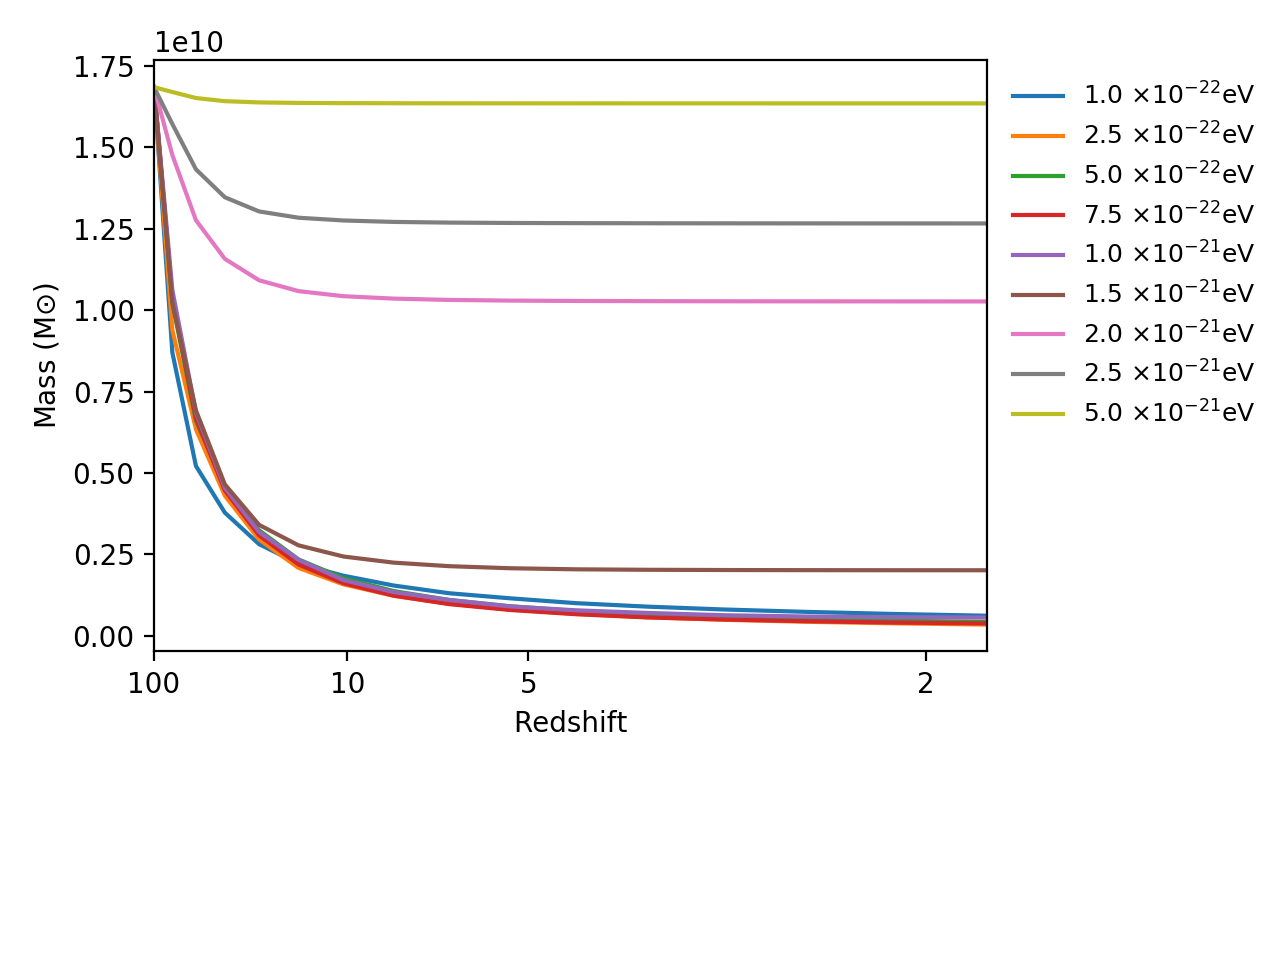
\includegraphics[trim={0cm 3cm 2cm 0cm},scale=0.8]{mass_loss_ULDM_mass.png}
  \caption{Mass loss due to gravitational cooling of a collapsing elliposidal top-hat overdensity for varying ULDM particle mass. Above $10^{-21}$eV, the gravitational cooling mechanism is rapidly suppressed. In all cases plotted, mass loss has decreased to approximately zero by $z=2$, indicating a stable final profile has been reached.}\label{fig:mass_loss_ULDM_mass}
\end{figure}

From Figure \ref{fig:mass_loss_ULDM_mass}, we see that for the ULDM particle mass range $10^{-22}$ to $10^{-21}$ eV, the final relaxed halos have approximately the same mass. However, as the de Broglie wavelength decreases, we expect that the solitonic cores of the halos become less pronounced, such that the overall density profile tends toward the NFW profile of CDM. Indeed, we see this behaviour demonstrated in Figure \ref{fig:profile_comp_with_sol}. For a ULDM particle mass of $10^{-22}$eV, we see a pronounced solitonic core, closely matching the theoretical soliton profile until approximately 4 times the radius at half-maximum density. As ULDM particle mass is increased, the density profiles tend toward a more NFW-like configuration. 

\begin{figure}[!htb]
    \centering
  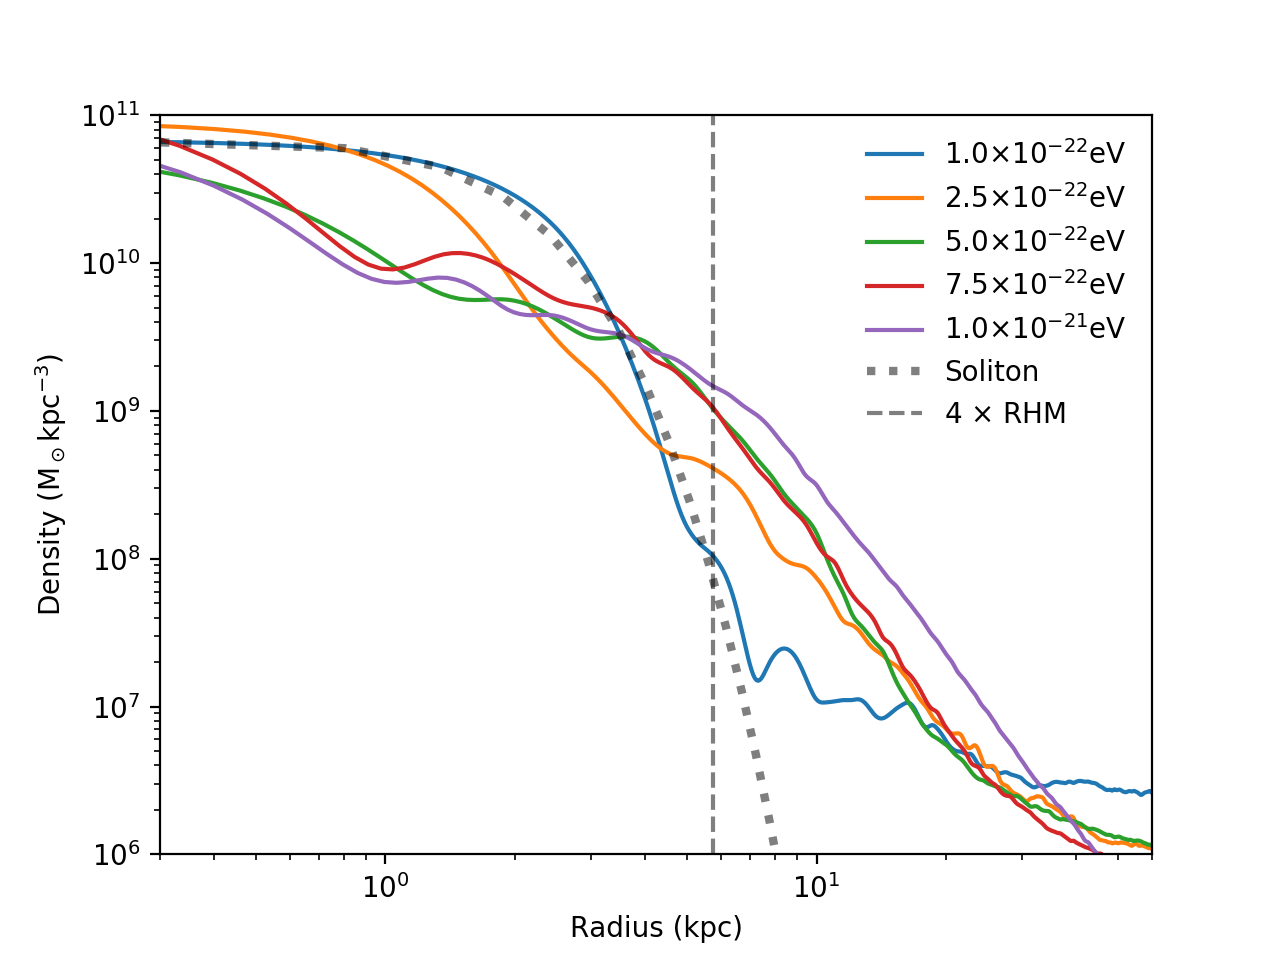
\includegraphics[trim={0cm 0cm 0cm .5cm},scale=0.7]{profile_comp_with_sol.png}
  \caption{Final spherically-averaged density profiles at $z = 1.5$. The halos have similar total mass but varying ULDM particle mass, resulting in differences in the profile shape. Plotted also is the solitonic profile for ULDM particle mass $10^{-22}$eV, and a corresponding vertical line indicating 4 times the radius at half maximum density.}\label{fig:profile_comp_with_sol}
\end{figure}

As wavelike behaviour is suppressed with increasing ULDM particle mass, we expect that interference fringes in the collapsing density profiles will become less pronounced. Figures \ref{fig:contours_21} and \ref{fig:contours_22} show the (log) density distributions through the central plane of the simulation region for ULDM particle masses $10^{-21}$eV and $10^{-22}$eV, respectively. In the left panels we show the density distributions at $z=97$, shortly after the onset of collapse. For ULDM mass $10^{-22}$eV, we can clearly see pronounced interference fringes emanating from the centre as Zel'dovich type collapse is impeded by wavelike behaviour. For ULDM mass $10^{-21}$eV, the fringes are much finer as a result of the decreased de Broglie wavelength. In the right panels of Figures \ref{fig:contours_21} and \ref{fig:contours_22}, we see the density contours for the final relaxed halos at $z\approx 1.5$. We see a much smoother distribution for the heavier ULDM particle mass, while the $10^{-22}$eV case exhibits turbulence in the outer halo on the scale of the larger de Broglie wavelength. 

In both figures, we can see artifacts of the cubic grid in the form of regular granularity and slightly higher densities along the principal grid axes. We anticipate that more advanced simulation tools currently in development, such as {\sc AxioNyx} \cite{Schwabe:2020eac}, will prove useful in ameliorating this problem. Such tools are able to make use of Adaptive Mesh Refinement (AMR) to provide much greater resolution in areas of interest, and are also able to simulate much larger volumes while preserving fidelity on small scales.


\begin{figure}[!htb]
\minipage{0.5\textwidth}
  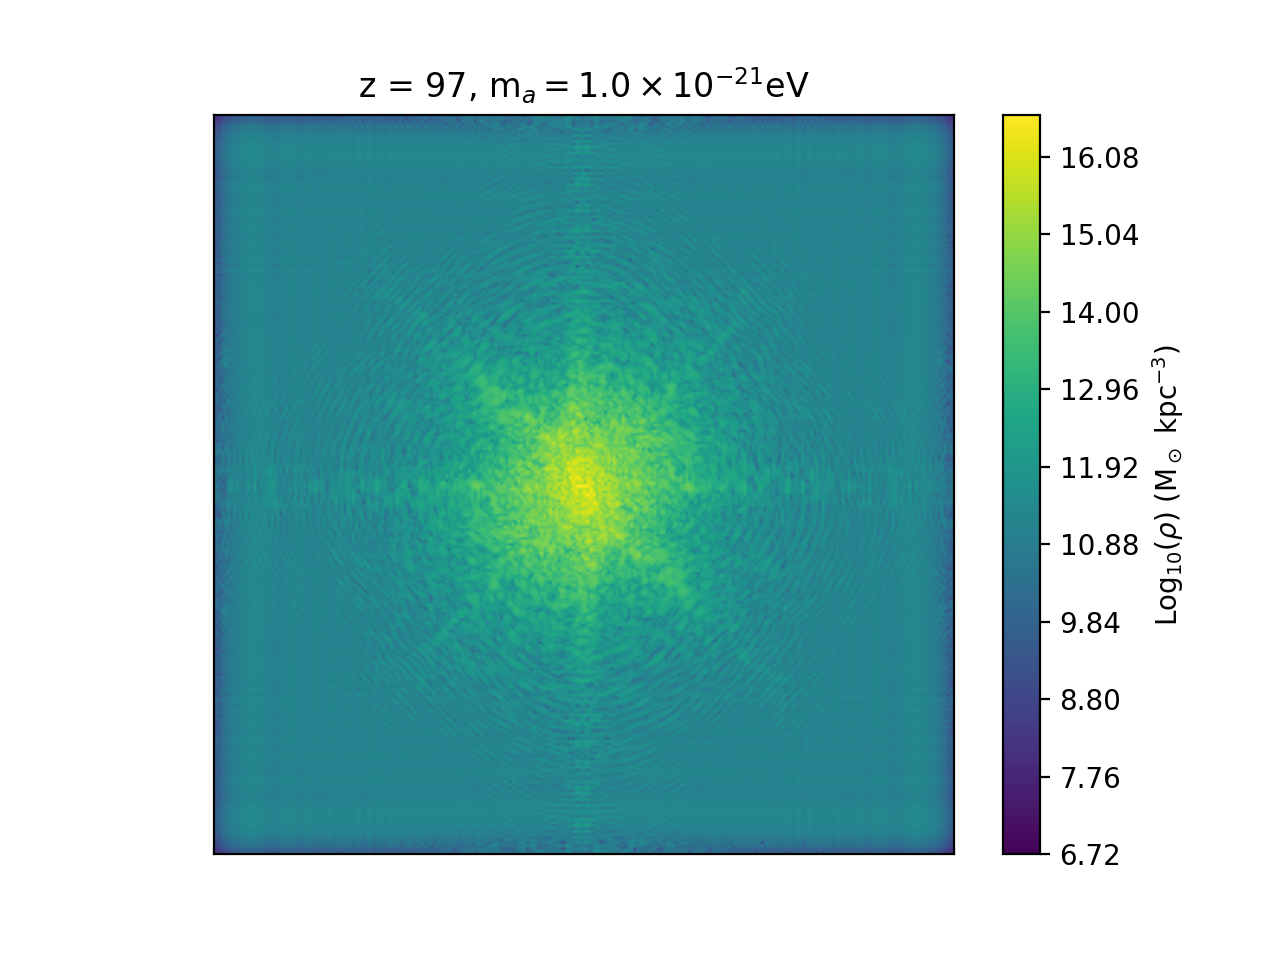
\includegraphics[trim={3cm 0 0 0}, scale=0.62]{z97_1e-21.png}
\endminipage\hfill
\minipage{0.5\textwidth}
  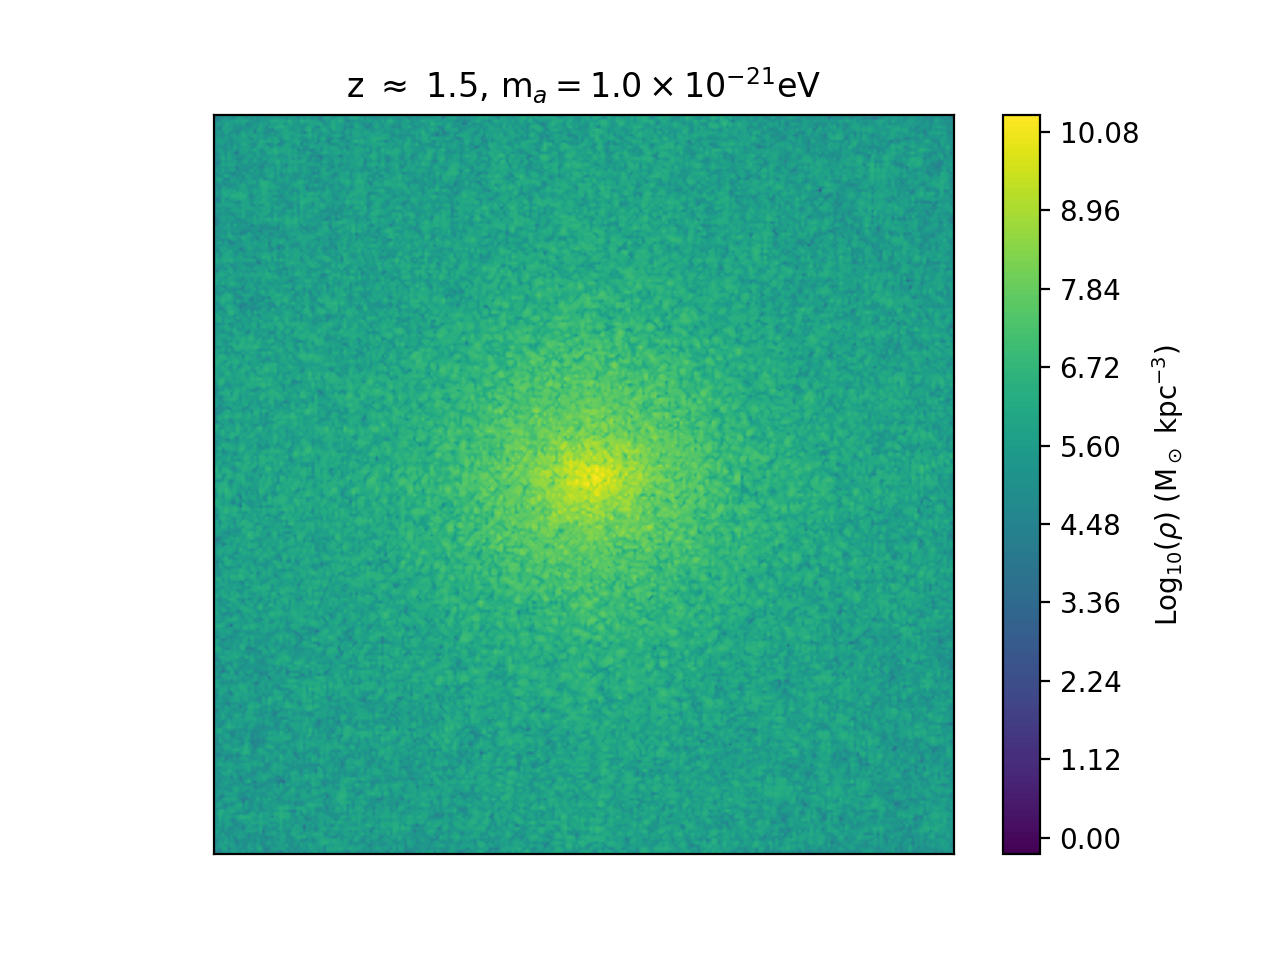
\includegraphics[trim={2cm 0 1cm 0},scale=0.62]{final_21.png}
\endminipage\hfill
\caption{Density contours through the centre of the simulation grid at $z=97$ (left) and $z\approx 1.5$ (right) for ULDM particle mass $10^{-21}$eV.}\label{fig:contours_21}
\end{figure}

\begin{figure}[!htb]
\minipage{0.5\textwidth}
  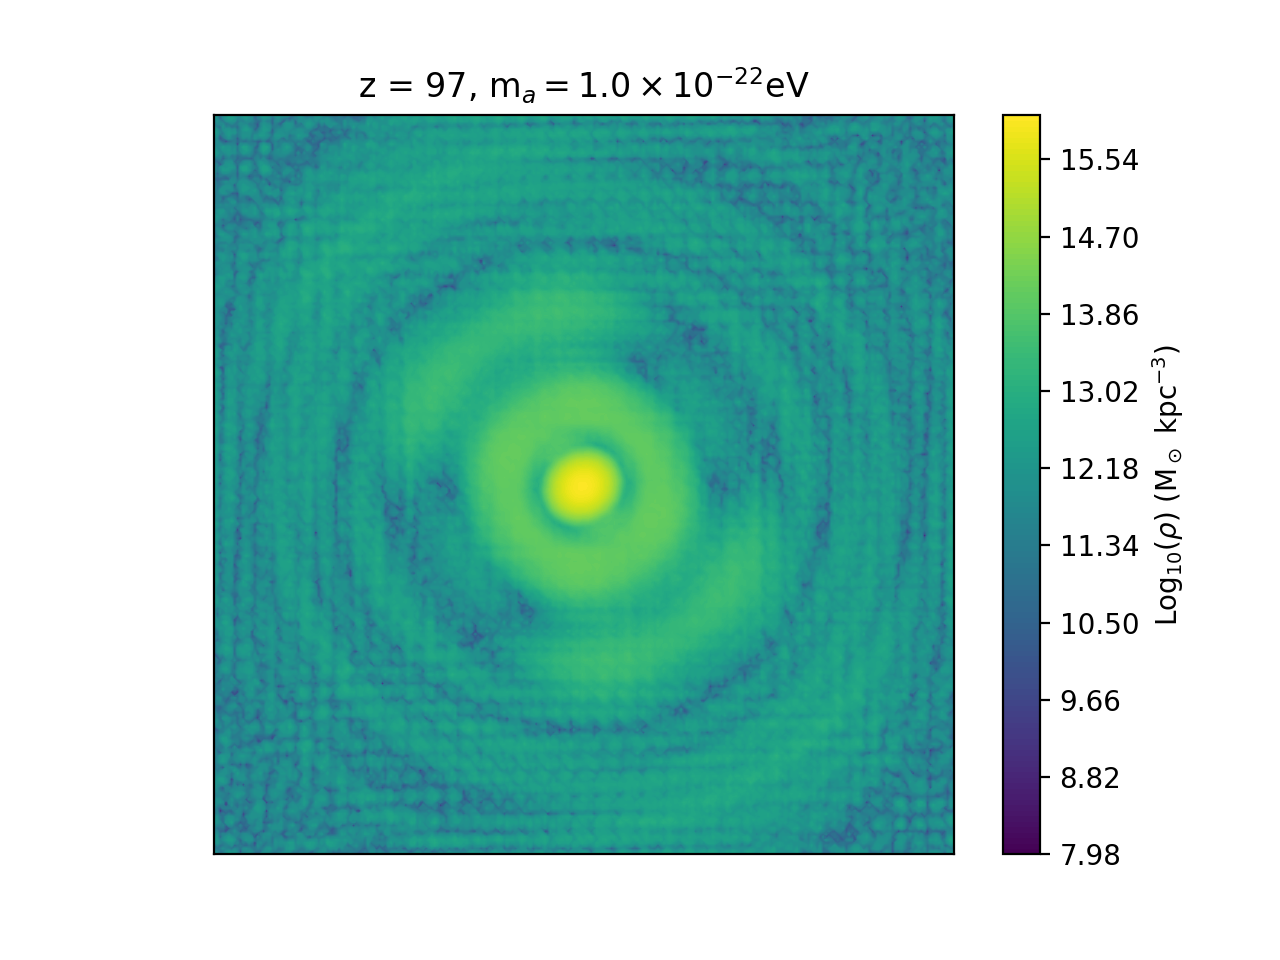
\includegraphics[trim={3cm 0 0 0}, scale=0.62]{z97_1e-22.png}
\endminipage\hfill
\minipage{0.5\textwidth}
  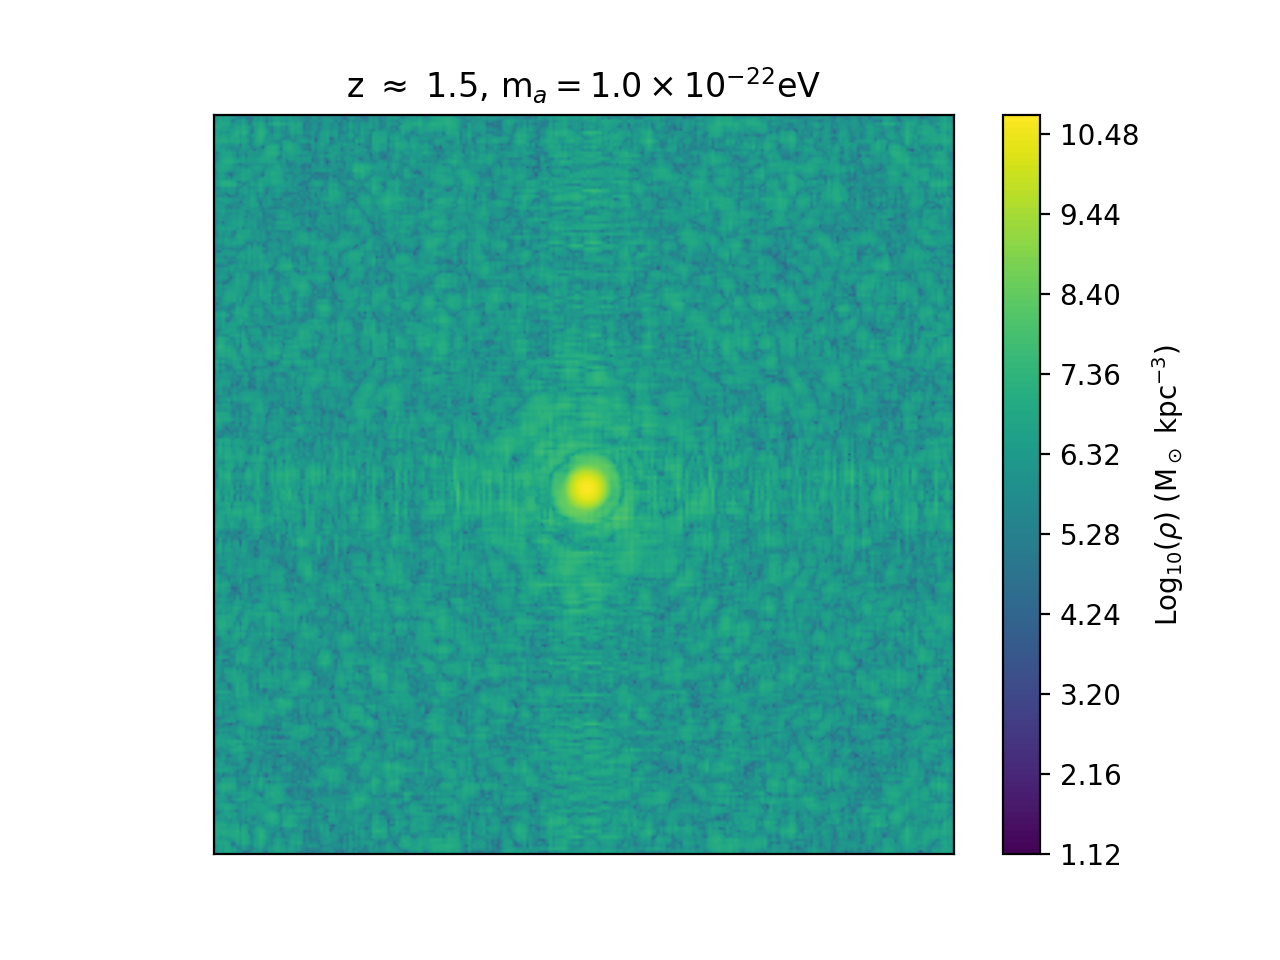
\includegraphics[trim={2cm 0 1cm 0},scale=0.62]{final_22.png}
\endminipage\hfill
\caption{Density contours through the centre of the simulation grid at $z=97$ (left) and $z\approx 1.5$ (right) for ULDM particle mass $10^{-22}$eV.}\label{fig:contours_22}
\end{figure}

While Figures \ref{fig:contours_21} and \ref{fig:contours_22} provide a visual demonstration of the differences in the collapse process for varying ULDM particle mass, it is of interest to also develop tools to quantify these differences. In order to demonstrate how this may be achieved, we provide here a proof-of-principle analysis of the statistics of the traceless tidal tensor (TTT) for the density distributions at $z=97$.

We motivate this analysis by the fact that high-resolution cosmological simulations seem to suggest that there may be additional structure present in the filaments of the cosmic web in the ULDM case compared to the CDM case, due to interference effects \cite{Mocz:2019emo}. Such extended anisotropies cannot be completely characterised using the 2-point correlator, and thus it may prove useful to examine the statistics of quantities which preserve information about anisotropy in density distributions, such as the tidal tensor. The traceless tidal tensor at each point in a density field gives the deformation of the corresponding volume element relative to purely spherical expansion or collapse. It is therefore an ideal tool to characterise fields in which structures possessing directional dependence arise. While we do not suggest that the results shown here can be directly applied to large scale cosmological structure, they serve to motivate the use of such statistical tools as a means by which to quantify the differences between ULDM and CDM density distributions and to possibly constrain the ULDM particle mass. 

Following \cite{Lee:2009uv}, from the density fields output by the {\sc PyUltraLight} simulation tool, we construct the traceless tidal tensor at each grid point. To do this, we first compute the dimensionless overdensity field:
\begin{equation}
    \delta(\mathrm{\mathbf{x}}) = \frac{\rho(\mathrm{\mathbf{x}})-\Bar{\rho}}{\bar{\rho}}, 
\end{equation}
where $\bar{\rho}$ is the average density throughout the simulation volume. We then take the Fourier transform to obtain the dimensionless density contrast in Fourier space, $\delta(\mathrm{\mathbf{k}})$. From here we can calculate the peculiar gravitational field from the Poisson equation, and finally compute the tidal tensor as the Hessian of the peculiar gravitational potential. In Fourier space we have
\begin{equation}
    \phi(\mathrm{\mathbf{k}}) = k^{-2}\delta(\mathrm{\mathbf{k}}), \qquad T_{ij}(\mathrm{\mathbf{k}}) = k_{i}k_{j}\phi(\mathrm{\mathbf{k}}).
\end{equation}
At each point, the dimensionless density contrast is given by the trace of the tidal tensor. Therefore, in order to isolate the tidal effects, we compute the Fourier space TTT:
\begin{equation}
    \Tilde{T}_{ij}(\mathrm{\mathbf{k}}) = T_{ij}(\mathrm{\mathbf{k}}) - \frac{\delta(\mathrm{\mathbf{k}})}{3}\mathbb{I}_{ij}.
\end{equation}
Finally we perform an inverse Fourier transform to obtain the TTT in real space. We then randomly select a sample of 15,000 points from the simulation grid at which to diagonalise the tidal tensor, storing the eigenvalues ($\lambda_1$, $\lambda_2$, $\lambda_3$) and unit eigenvectors ($\mathrm{\mathbf{e}}_1$, $\mathrm{\mathbf{e}}_2$, $\mathrm{\mathbf{e}}_3$) for further analysis. We label the eigenvalues such that $\lambda_1 >\lambda_2 > \lambda_3$. Because these are the eigenvalues of the \textit{traceless} tensor, we also have $\lambda_1>0$ and  $\lambda_3 < 0$, while $\lambda_2$ may be either positive or negative.

Having obtained the eigenvalues of the TTT, we may examine their probability distributions for different ULDM masses. In this case we will consider the density distributions illustrated in Figures \ref{fig:contours_21} and \ref{fig:contours_22} at $z=97$. In general, we expect the presence of repeated anisotropic structures such as wavefronts to induce peaks in the probability distributions of the eigenvalues, as in such cases there will be a number of volume elements exhibiting the same characteristic anisotropic deformation. In Appendix \ref{app:prob_distro_eg} we demonstrate this effect using artificial density distributions. 

Because the traceless tidal field was computed for 15,000 randomly chosen points within the simulation grid, there are a total of 45,000 data points from which to construct the probability distributions of the three eigenvalues. Because we have a finite number of samples, we must choose a smoothing method to obtain a continuous distribution. In this case, we divide the eigenvalue range $\{-3,+3\}$ into 1000 bins, tallying the number of points which fall into each bin. We represent the outcome of this procedure using the scattered points in Figure \ref{fig:prob_distros}. In order to gauge the presence of peaks in the distribution, we overlay these points with a best-fit cubic spline interpolation. The degree of smoothing will of course affect the visible level of substructure, however we note that the smoothing procedure applied here is sufficient to identify qualitative differences in the probability distributions of the $10^{-22}$eV and $10^{-21}$eV cases. 

\begin{figure}[!htb]
\centering
\minipage{0.5\textwidth}
  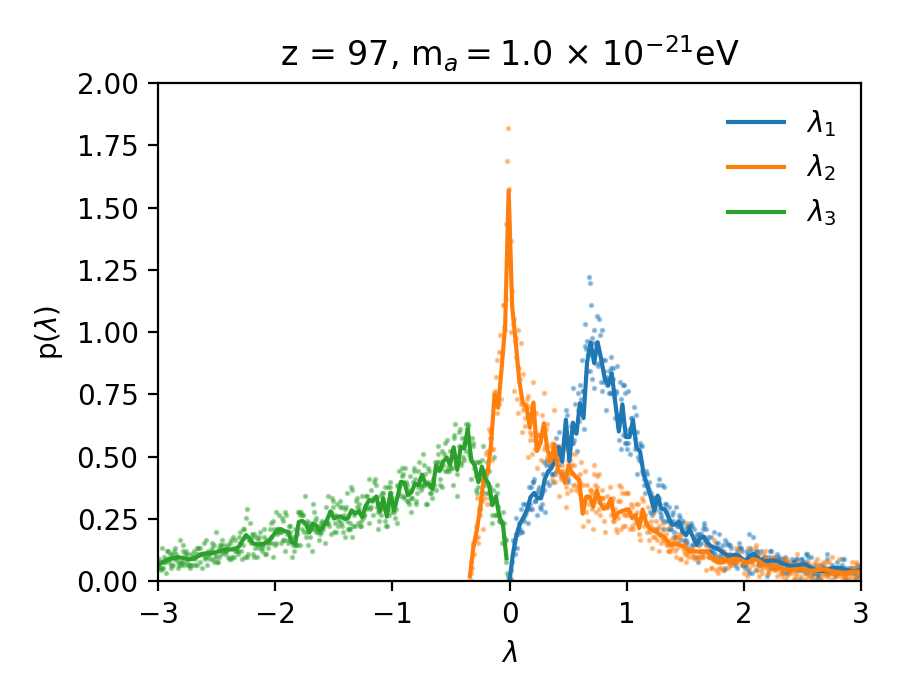
\includegraphics[trim={1cm 0 2cm 0.2cm},scale=0.75]{ev_z97_1e-21.png}
\endminipage\hfill
\minipage{0.5\textwidth}%
  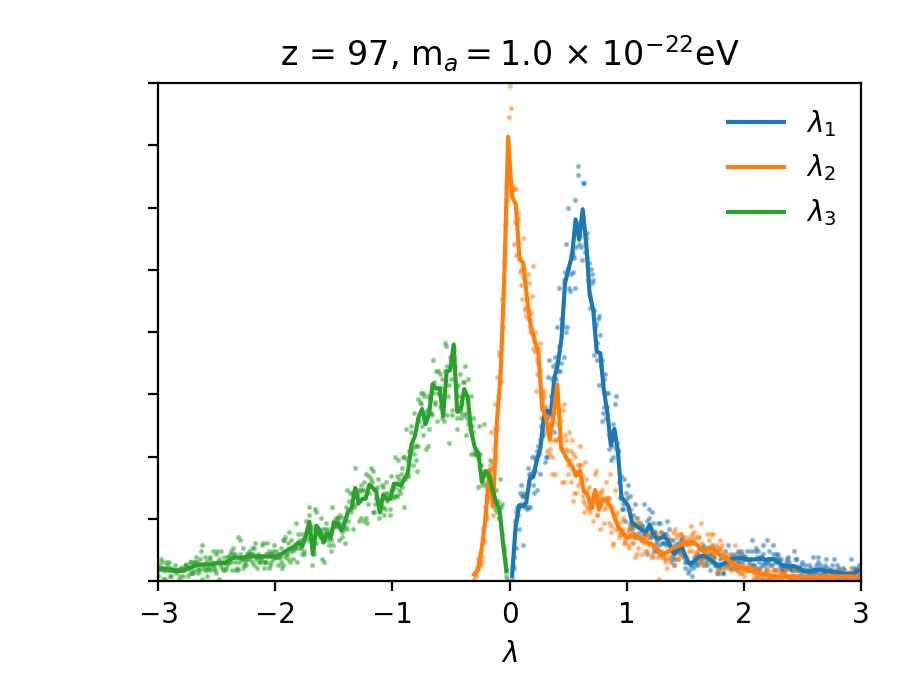
\includegraphics[trim={1cm 0 2cm 0.1cm},scale=0.75]{ev_z97_1e-22.png}
\endminipage
\caption{Probability distributions of the eigenvalues of the traceless tidal tensor near the onset of collapse ($z=97$) for m$_a = 10^{-21}$eV (left) and m$_a = 10^{-22}$eV (right).}\label{fig:prob_distros}
\end{figure}

Our results are presented in Figure \ref{fig:prob_distros}. For ULDM particle mass $10^{-22}$eV, we see a generally more peaked distribution, with the appearance of enhanced substructure in the distribution of the third eigenvalue. The distributions for the $10^{-21}$eV case are more spread out and exhibit greater symmetry between the first and third eigenvalues, indicative of a smoother density distribution with less pronounced extended anisotropies. 

These results, while preliminary, show that the TTT may serve as a useful quantitative tool for characterising the substructure of density distributions arising during gravitational collapse in ULDM models. Further investigation, including a detailed analysis of the anisotropic 2-point correlation functions of the eigenvalues of the TTT are planned for future work, when the outputs of more sophisticated ULDM simulations become available.


\section{Collapse and gravitational cooling of ellipsoidal overdensities for varying size and ellipticity}\label{sec:ellipticity}

In the previous section, we considered only the effect of varying the ULDM particle mass on the collapse of ellipsoidal overdensities. In this section, we keep the ULDM particle mass constant at $10^{-22}$eV, but vary both the shape and size of the initial overdensity. We then compare the rates of mass loss via gravitational cooling and the properties of the final relaxed profiles. 

We refer back to the initial configuration used in Section \ref{sec:sims}. That is, we define our ellipsoidal overdensity through Equations \ref{eq:ellipse} and \ref{eq:flattening}. We vary the parameters $R$ and $f$ in order to change the volume and flattening, respectively. We define $R$ in terms of a multiple of the grid resolution for convenience, choosing from the following four factors: (0.5, 1.0, 2.0, 3.0). We vary the parameters ($a, b, c$) under the constraints $a \times b \times c = 1$ and $a = b$ to obtain the following four flattening values: (0.0, 0.25, 0.5, 0.75). As in Section \ref{sec:ULDM_mass}, we choose a top-hat overdensity of $2500a(t)^{-3}$ code units, and a simulation side length of $10a(t)$ code units. The mass of the overdensity varies only with the choice of $R$, such that our initial overdensities have masses ($2.0\times 10^9$, $5.7\times 10^9$, $1.6\times 10^{10}$, $2.9\times 10^{10}$) M$_\odot$ for $R = $ (0.5, 1.0, 2.0, 3.0)$\times \mathrm{Res}$ at  $z=100$. We then combine the possibilities for $R$ and $f$ for a total of 16 different initial configurations. For each mass, we find that the initial rate of mass loss through gravitational cooling is highest for the spherical configuration, and decreases as the flattening increases. Correspondingly, at the end of the simulation, those overdensities with higher initial flattening lead to relaxed halos of higher mass. We present two representative mass loss plots as functions of flattening and volume in Figure \ref{fig:mass_loss_flat_size}, noting that the same dependencies are observed for different parameter combinations.

\begin{figure}[!htb]
\centering
\minipage{0.5\textwidth}
  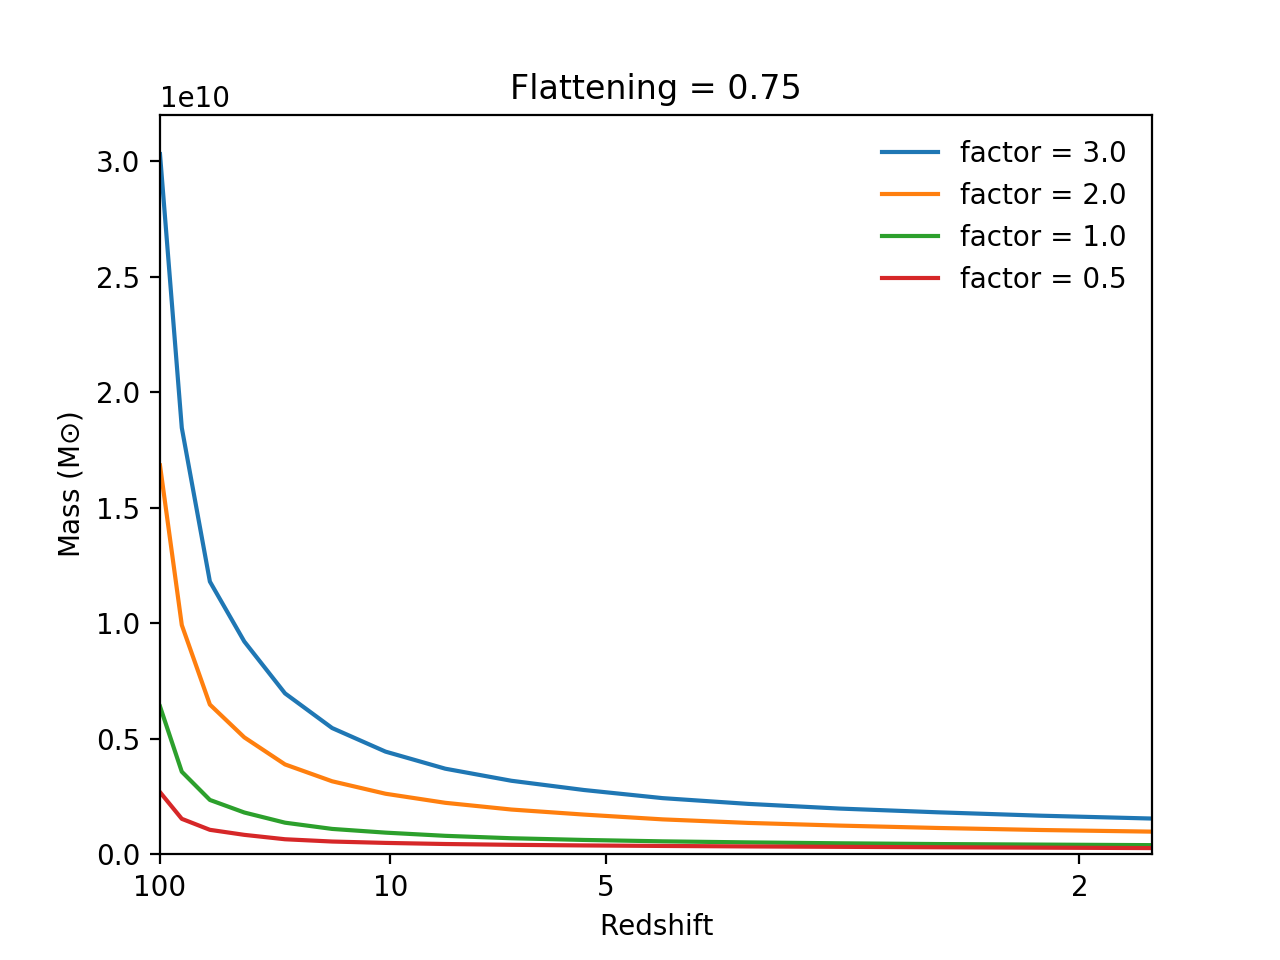
\includegraphics[trim={1cm 0 2cm 0.2cm},scale=0.55]{mass_loss_0_75.png}
\endminipage\hfill
\minipage{0.5\textwidth}%
  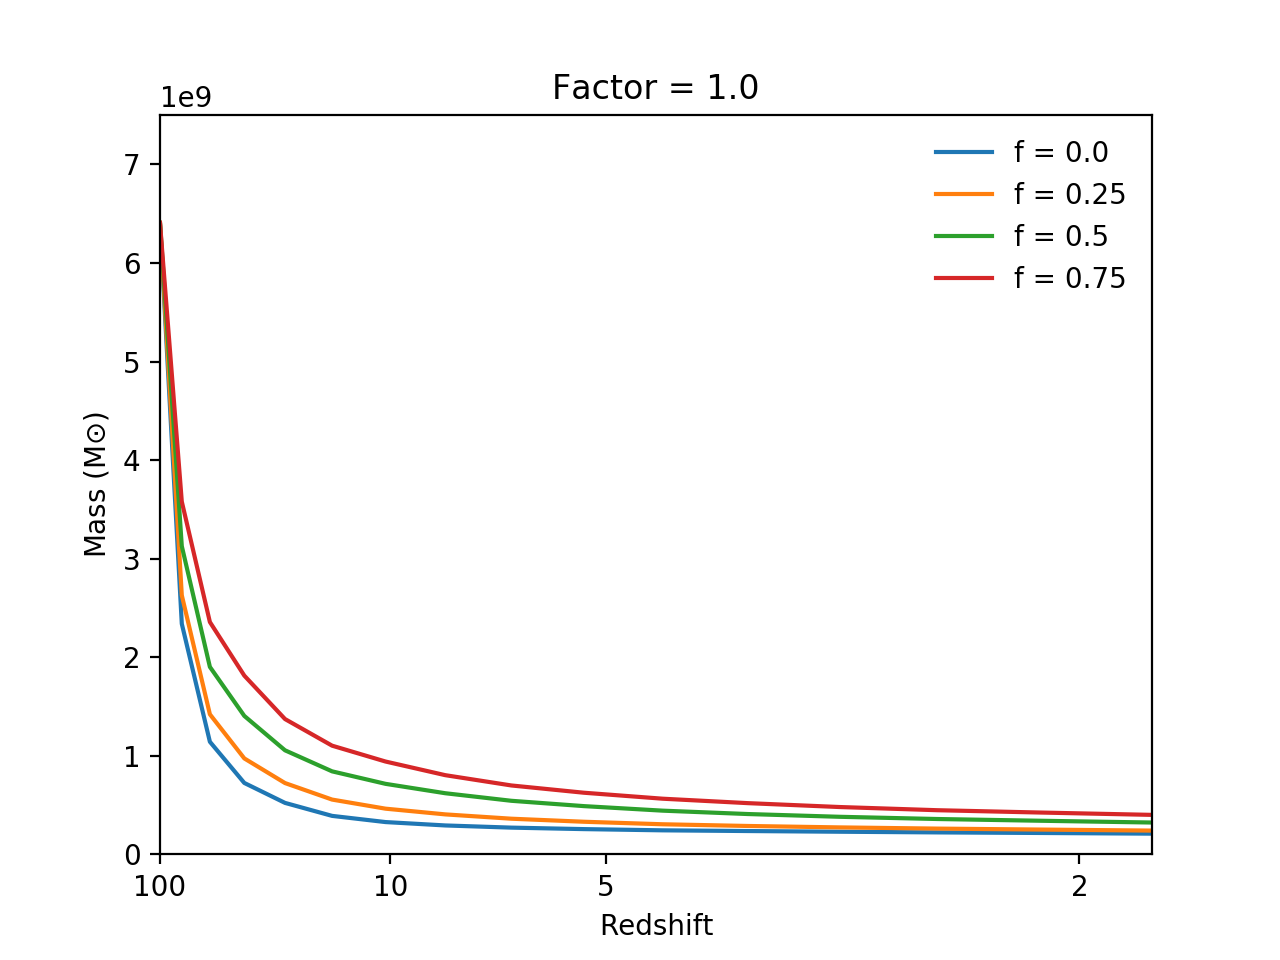
\includegraphics[trim={0.2cm 0 2cm 0.1cm},scale=0.55]{mass_loss_f_1.png}
\endminipage
\caption{Left: mass loss as a function of $R$ (given as a (factor) multiple of the grid resolution) for $f = 0.75$. Right: mass loss as a function of the flattening parameter $f$ for $R = 1 \times \mathrm{Res}$. Similar behaviour is exhibited for different $R$ and $f$ values.}\label{fig:mass_loss_flat_size}
\end{figure}

Figure \ref{fig:mass_loss_flat_size} demonstrates that the gravitational cooling rates depend on both the size and shape of the initial overdensity. To determine the impact of this on the final relaxed halos, we plot each of the 16 spherically-averaged density profiles at $z=1.5$ in the left panel of Figure \ref{fig:profiles_combined}. 

\begin{figure}[!htb]
\centering
\minipage{0.5\textwidth}
  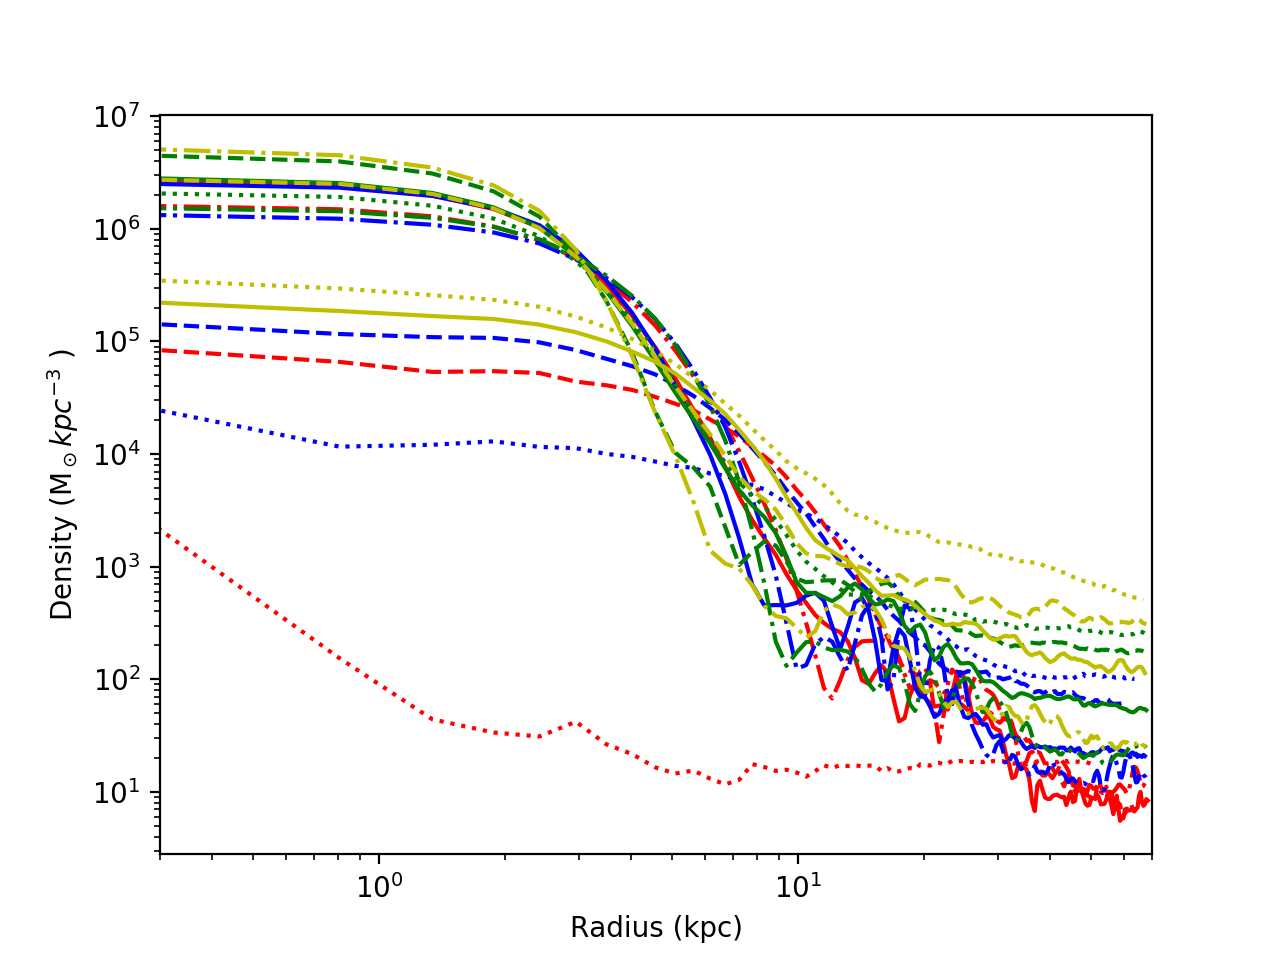
\includegraphics[trim={1cm 0 2cm 0.2cm},scale=0.55]{profiles_combined.png}
\endminipage\hfill
\minipage{0.5\textwidth}%
  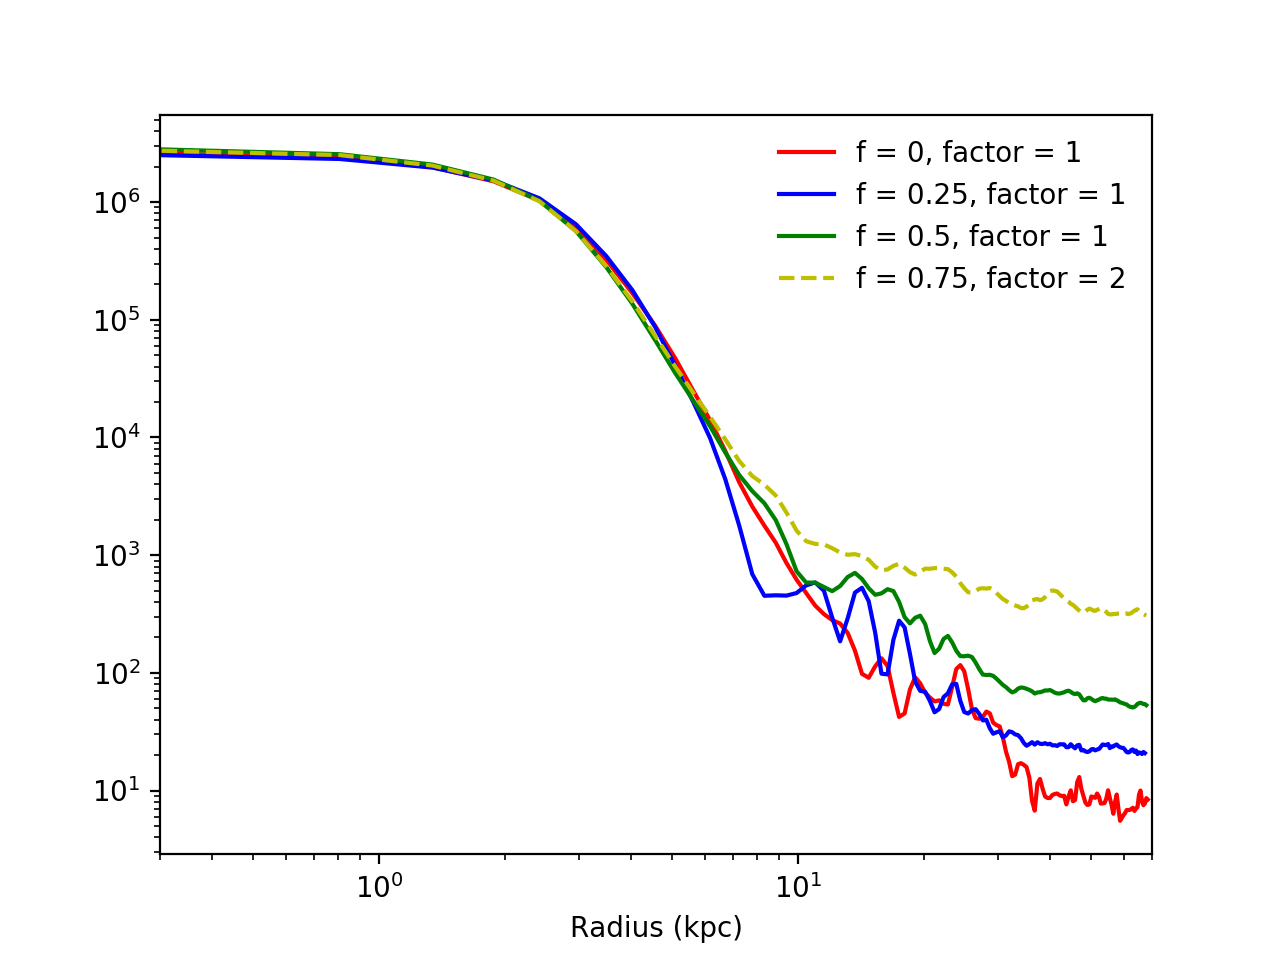
\includegraphics[trim={1cm 0 2cm 0},scale=0.55]{profiles_selected.png}
\endminipage
\caption{Left: spherically averaged density profiles at $z=1.5$ for different $f$ and $R$ parameters. Here ($f = 0.0$, $f=0.25$, $f=0.50$, $f=0.75$) $\rightarrow$ (red, blue, green, yellow) and ($R=0.5\times\matrm{Res}$, $R=1\times\matrm{Res}$, $R=2\times\matrm{Res}$, $R=3\times\matrm{Res}$) $\rightarrow$ (dot-dashed, solid, dashed, dotted). Right: a selection of final profiles with similar cores but differing outer halo behaviour.}\label{fig:profiles_combined}
\end{figure}

In the left panel of Figure \ref{fig:profiles_combined}, we see that for large initial overdensities with zero flattening (red and blue dotted lines), too much mass is lost from the simulation region via gravitational cooling to form a stable core-halo type final configuration. However, for smaller initial volumes or larger flattening parameters, we obtain a variety of profiles exhibiting the characteristic core-halo configuration of ULDM. Interestingly, however, there are a number of halos which, while possessing almost identical cores, exhibit significant variations in the outer halo. We isolate four such profiles in the right panel of Figure \ref{fig:profiles_combined}. As shown in the figure, these arise from each of the four different initial flattening values, and for both $R = 1\times\mathrm{Res}$ and $R = 2\times\mathrm{Res}$, indicating that a combination of initial conditions is responsible for determining the shape of the final halo. For the four profiles isolated in the right panel of Figure \ref{fig:profiles_combined}, each has a core mass of $1.1\times 10^{8}$M$_\odot$, while the outer halo masses are $2.0\times 10^{8}$M$_\odot$, $2.2\times 10^{8}$M$_\odot$, $2.6\times 10^{8}$M$_\odot$, and $6.7\times 10^{8}$M$_\odot$. Here the core is defined as the region within which the density is greater than $1/2$ of the peak central density. 

This variation halo profile characteristics suggests a source of variability in the widely cited theoretical core-halo mass relation of ULDM \cite{Schive:2014hza}. In this case, the outer halos vary by a factor of $>3$ in total mass within the plotted region. We note that the physical size of our simulation regions are limited by the fixed spatial resolution, and as such, more advanced simulations in which a larger portion of the outer profile were accessible would be desirable. However, these results seem to support other recent research in this area. In \cite{Nori:2020jzx}, the authors find that the theoretical core-halo scaling relations seem to be valid only as a limit for the most relaxed and spherically symmetric systems. 

We note, however, the inherent difficulties in verification of the core-halo mass relation. In particular, the `spatial extent' of a halo is ill-defined, with common approaches to approximate the virial radius as the point at which the average internal density is given by $\Delta\rho_c$, where $\rho_c$ is the critical density of the universe, and $\Delta$ is a factor of order 200. Different conventions are often employed here, making exact comparisons difficult. Furthermore, whether or not a halo may be considered to be truly `relaxed' is another source of uncertainty. For example, one may envisage a situation in which a `relaxed' halo comes under the gravitational influence of another object, distorting its density profile. Given these issues, further studies are planned in which we will numerically investigate the virialisation of simulated halos in differing density backgrounds in order to determine how the profiles may depend on various external factors and initial conditions. 


\section{Effect of angular momentum on overdensity collapse}\label{sec:rotation}

In this section, we augment the previous simulation setups by adding a varying phase parameter in order to generate angular momentum in the initial overdensities. To do this, we first create a gaussian profile for the magnitude of the phase parameter, concentric with the initial overdensity. The Gaussian profile is determined by three parameters, $\{g, \bold{b}, c\}$ through

\begin{equation}\label{eq:gauss}
    f(\bold{x}) = g\exp\left(-\frac{(\bold{x}-\bold{b})^2}{2c^2}\right)    
\end{equation}

We then distort this spherical gaussian profile to create an ellipsoidal profile with the same three axis parameters as the overdensity itself. However, we offset the orientations of the two ellipsoids by a non-zero angle. We then assign a phase $\theta$ to each field point, with the magnitude of the phase determined by the distorted Gaussian magnitude $f(\bold{x})$ at that grid position. That is,  

\begin{equation}
    \psi \rightarrow \psi \times \exp(i\theta),
\end{equation}
\\
where $\theta$ is determined by the magnitude of the distorted Gaussian. Because the velocity of the ULDM field is given by $\bold{v} = \bold{\nabla} \theta$, this process imparts rotational velocity to the original ellipsoidal overdensity. By varying the magnitude of the Gaussian parameter $a$ in Equation \ref{eq:gauss}, we can change the magnitude of the angular momentum of the overdensity.

We note that because we allow mass to be ejected from the simulation grid, we do not conserve angular momentum. Furthermore, the periodic boundary conditions of {\sc PyUltraLight} do not allow for conservation of angular momentum by definition. Thus, the study of the intrinsic rotation of the field presented here allows for a qualitative understanding of the distribution of angular momentum during overdensity collapse, but cannot yield a comprehensive quantitative analysis. 

To initialise the simulation, we use the same setup as described in the previous sections, namely, a simulation resolution of $\mathrm{Res} = 256$, $R = 2 \times \mathrm{Res}$ and flattening parameter $f=0.5$. The side length of the simulation region is set to $10a(t)$ code units and the density within the ellipsoid is set to $\rho = 2500a(t)^{-3}$ code units at $z=100$. This corresponds to an initial ellipsoidal overdensity of mass $1.6 \times 10^{10}$M$_\odot$. We then superimpose the distorted Gaussian phase field, offset from the overdensity by an angle of 1 radian. We choose parameters $\boldmath{b} = 0$ (no offset) and $c = 0.5$ for Equation \ref{eq:gauss}. We keep these parameters constant, but vary the value of the parameter $g$, to obtain differing rotational velocities. We choose $g = \{0.0, 2.5, 5.0, 7.5, 10.0\}$ for 5 separate runs, from $z=100$ to $z=1.5$. 

We compare the mass loss rates, the final spherically-averaged profiles, and the internal velocity distributions in each case. In addition, we provide visualisations of the overdensities near the onset of collapse for the lowest, middle, and highest values of $g$ in Figure \ref{fig:rotation_contours}. We see that as the initial angular momentum is increased, the wavefronts emanating from the centre of the simulation region become distorted. 


\begin{figure}[!htb]
\minipage{.3\textwidth}
  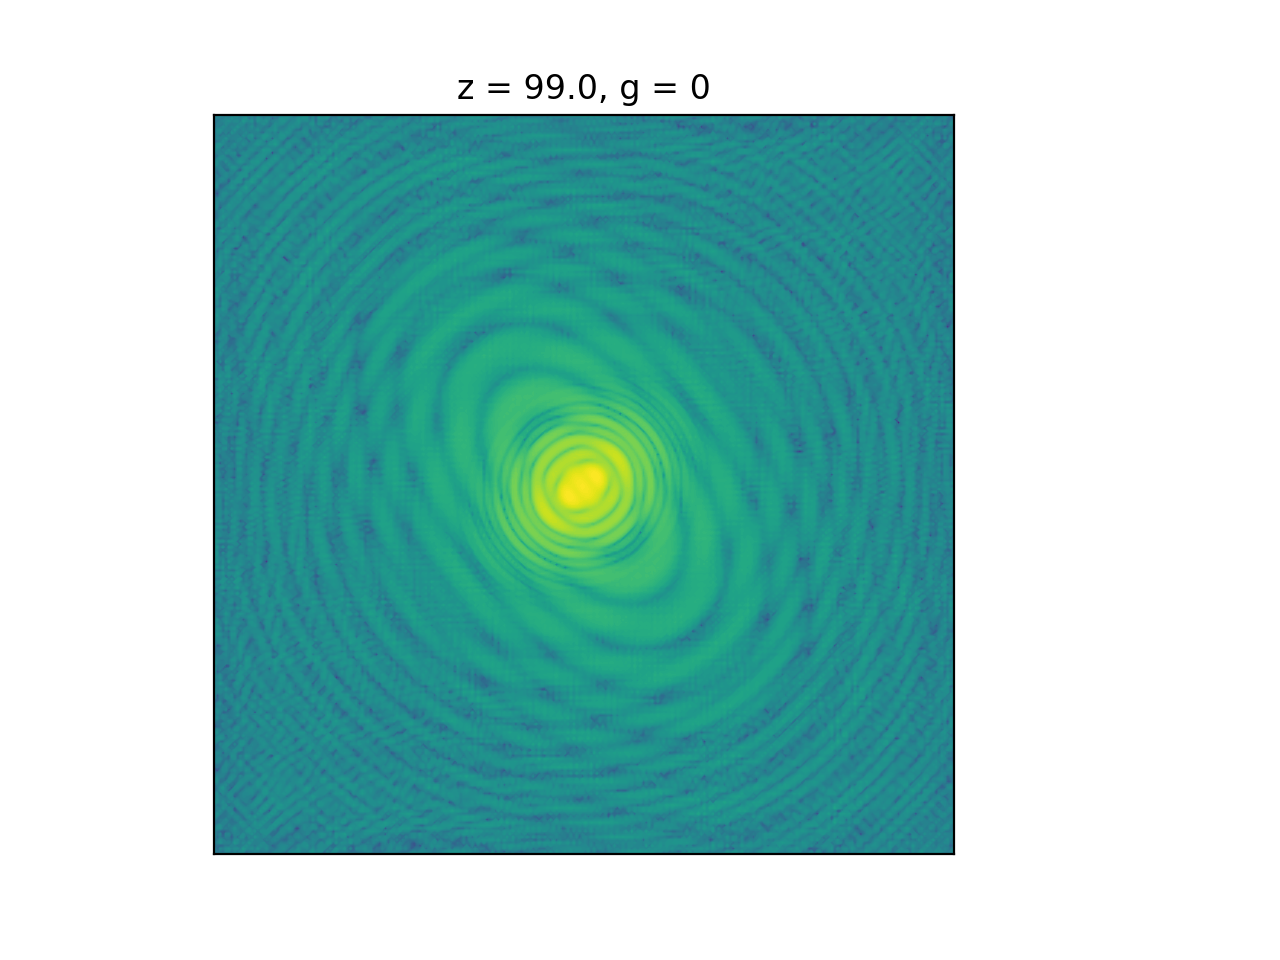
\includegraphics[trim={3cm 0 1cm 0cm},scale=0.52]{z_99_0_0.png}
\endminipage\hfill
\minipage{.3\textwidth}
  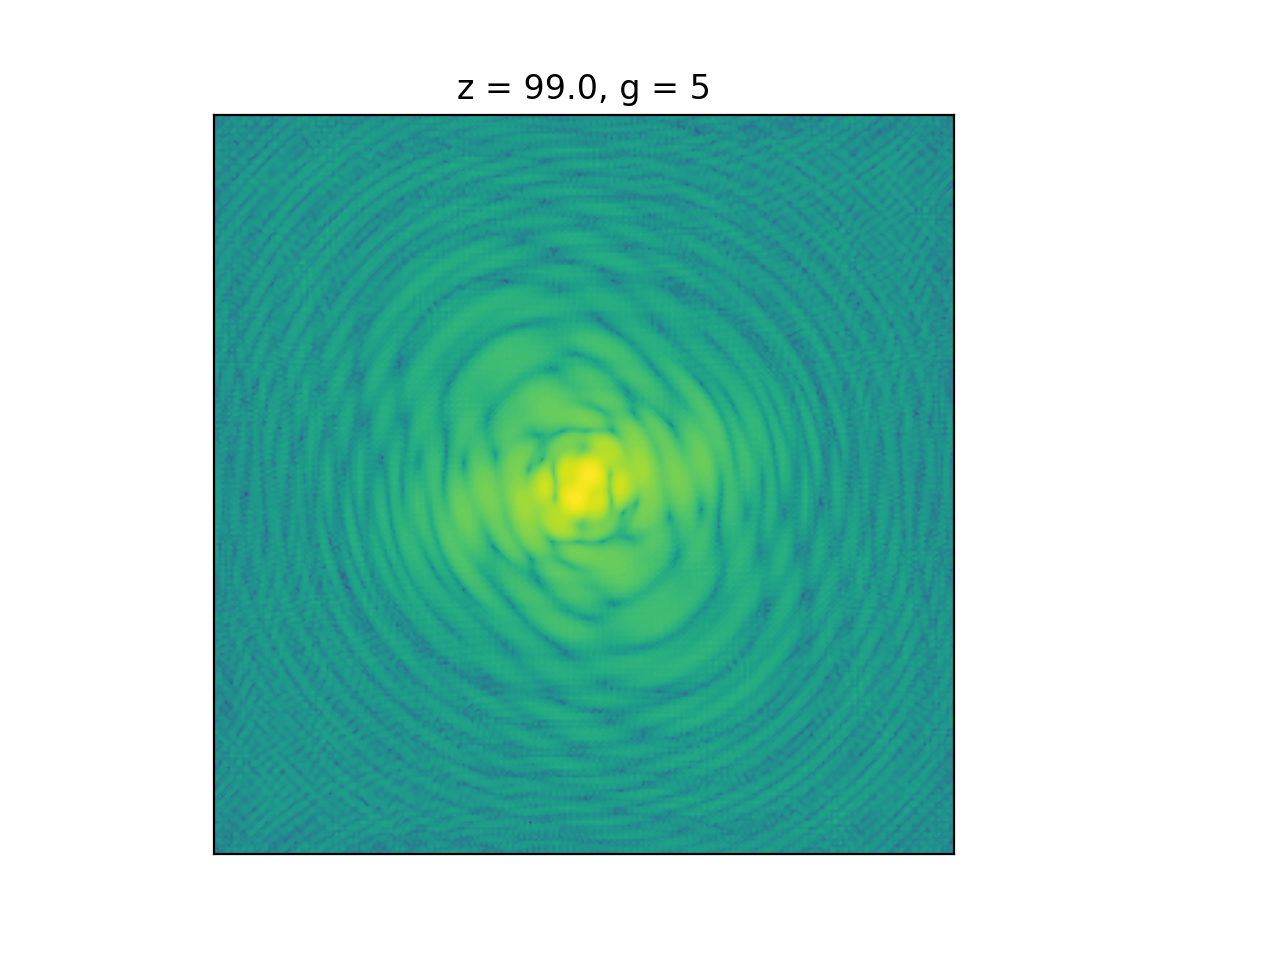
\includegraphics[trim={3.5cm 0 1cm 0cm},scale=0.52]{z_99_0_5.png}
\endminipage\hfill
\minipage{.3\textwidth}
  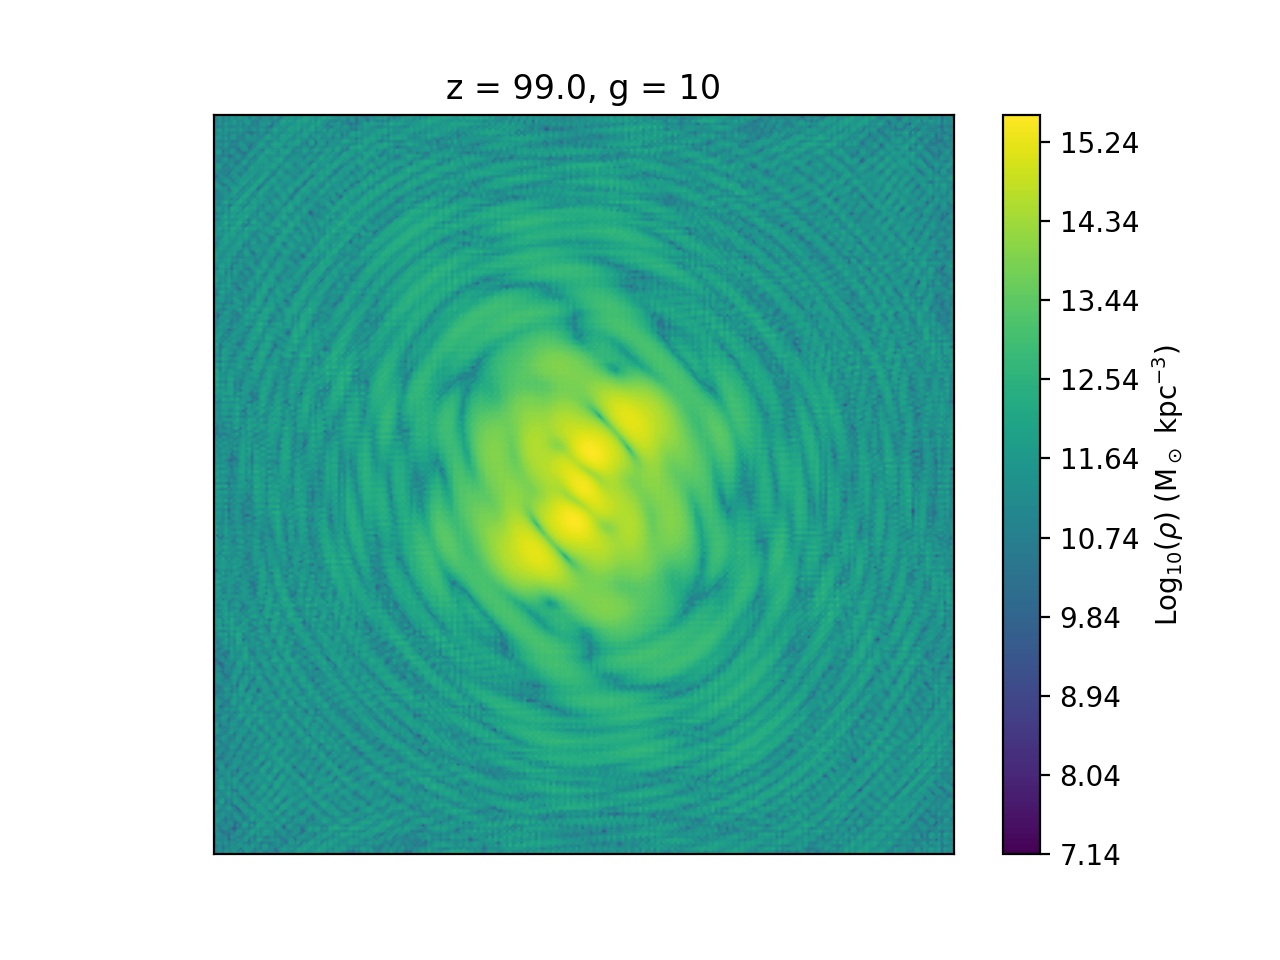
\includegraphics[trim={4.0cm 0 0cm 0cm},scale=0.52]{z_99_0_10.png}
\endminipage\hfill
\caption{Contours of density fields through the centre of the simulation region shortly after the onset of collapse ($z=99$). The initial angular momentum is increased as $g$ increases from $0$ to $10$, resulting in distortion of the outbound wavefronts.}
\label{fig:rotation_contours}
\end{figure}

In Figure \ref{fig:profiles_mass_rotation}, we compare the final spherically-averaged density profiles and the mass loss rates for varying $g$. In the case of the mass loss, increasing the initial angular momentum corresponds to a decrease in the overall mass loss, however above $g = 5.0$ this appears to stabilise, with the final masses for $g = 5.0$, $7.5$, and $10.0$ approximately equal. 

Interestingly, however, we do not observe a uniform change in the shape of the final profile as $g$ is increased. While each profile possesses a characteristic solitonic core, the central densities for $g = 2.5$ and $g = 10.0$ are the highest, and approximately equal. The central densities for $g = 0.0$ and $g = 7.5$ are somewhat lower, but also approximately equal. Finally, the central density for $g = 5.0$ is markedly lower than the other profiles.  

\begin{figure}[!htb]
\centering
\minipage{0.5\textwidth}
  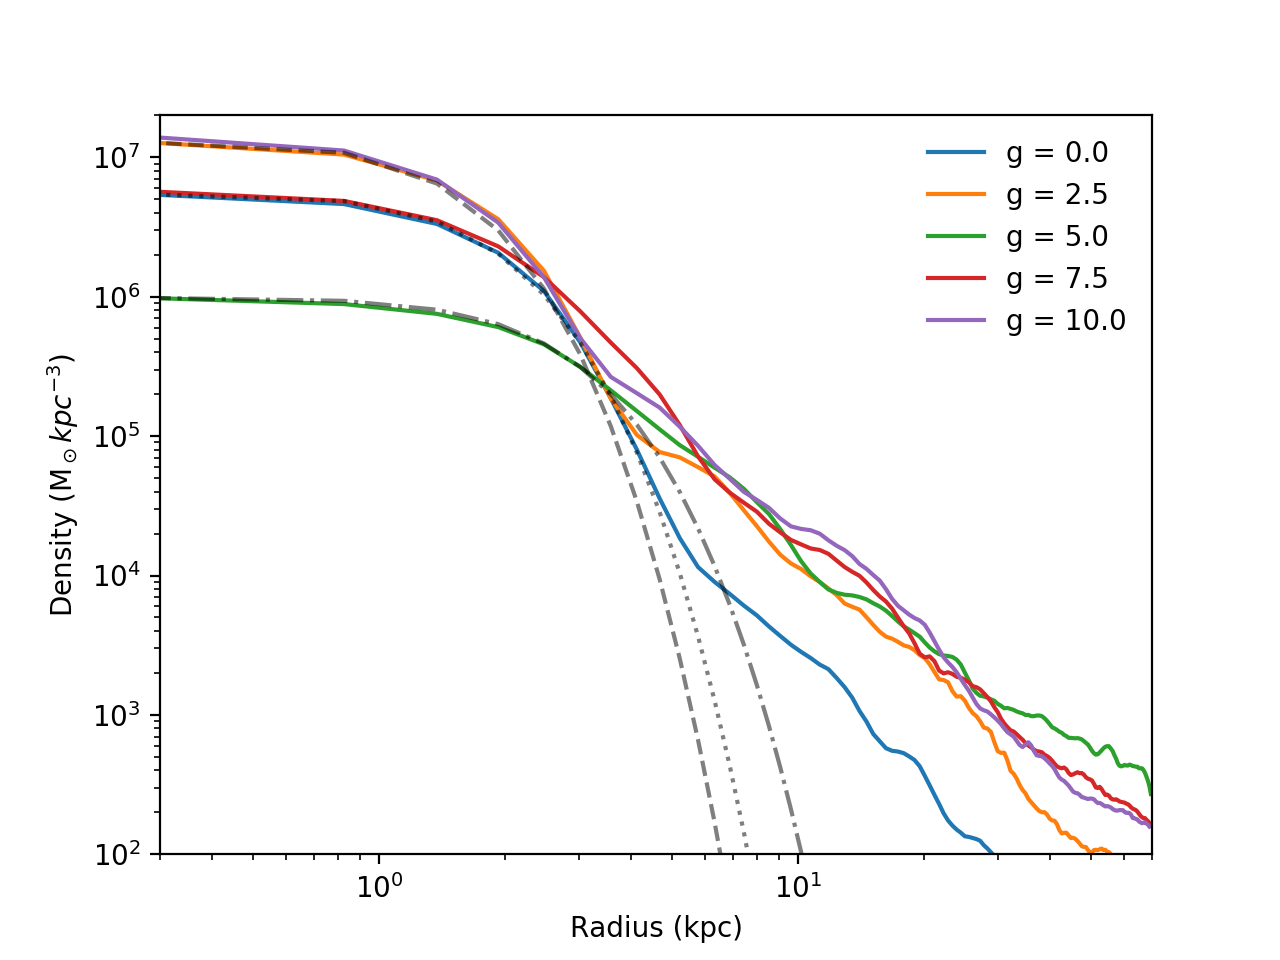
\includegraphics[trim={1.5cm 0 2cm 0.2cm},scale=0.55]{profiles_rotation.png}
\endminipage\hfill
\minipage{0.5\textwidth}%
  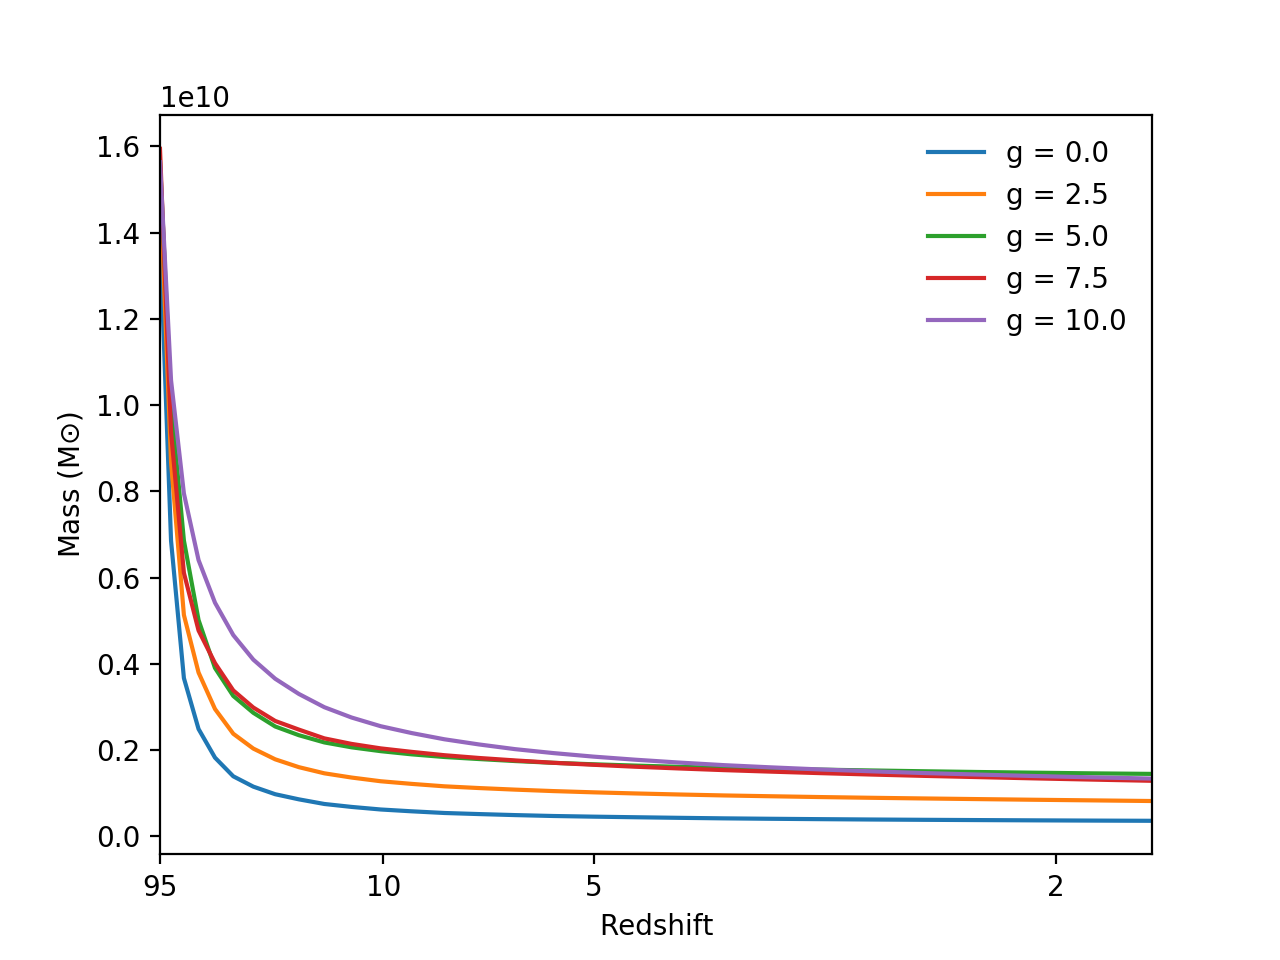
\includegraphics[trim={0.5cm 0 2cm 0},scale=0.55]{mass_loss_rotation.png}
\endminipage
\caption{Left: Final spherically-averaged density profiles for varying $g$ at $z=1.5$. Soliton profiles are shown in grey. Right: Mass loss rates via gravitational cooling for varying $g$.}\label{fig:profiles_mass_rotation}
\end{figure}

The final profiles shown in Figure \ref{fig:profiles_mass_rotation} serve as yet more evidence for variation around the theoretical core-halo mass relation, as halos with similar central densities possess disparate outer halo profiles. This indicates the presence of complicated collapse dynamics for rotating overdensities. It is as yet unclear why the $g=5.0$ case results in a markedly lower central density than both the smaller and larger $g$ values, and an investigation of the full dynamics of collapse will be the subject of future work, which may utilise more advanced AMR tools \cite{Schwabe:2020eac}.

In order to assess the affects of the initial angular momentum imparted to the ellipsoidal overdensities, we illustrate the internal velocity distributions near the onset of collapse and after relaxation in Figures \ref{fig:vels_initial_final} and \ref{fig:vels_final_contours}.


\begin{figure}[!htb]
\minipage{.3\textwidth}
  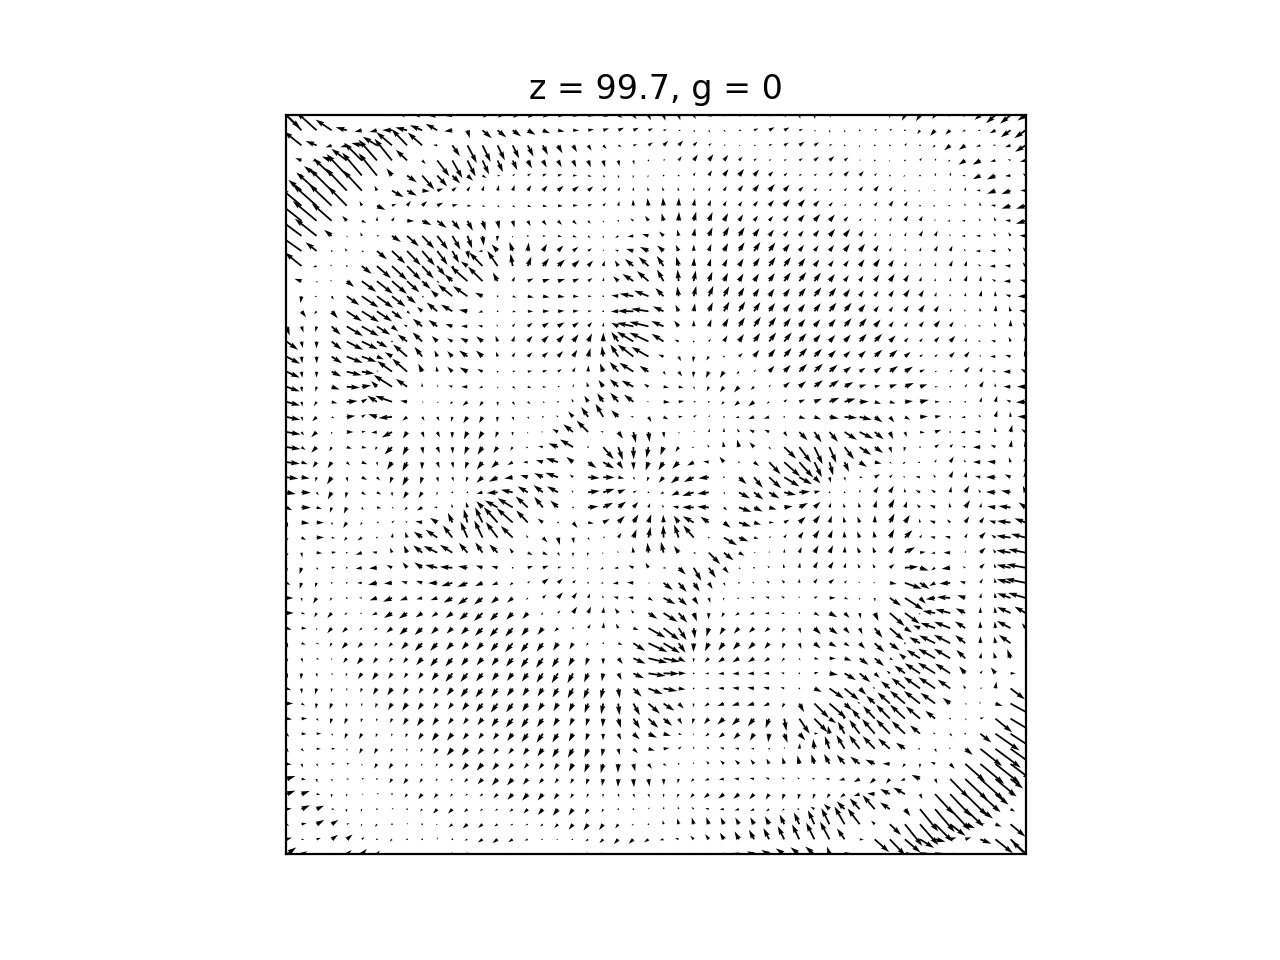
\includegraphics[trim={4cm 0 1cm 0cm},scale=0.5]{vel_99_7_g0.png}
\endminipage\hfill
\minipage{.3\textwidth}
  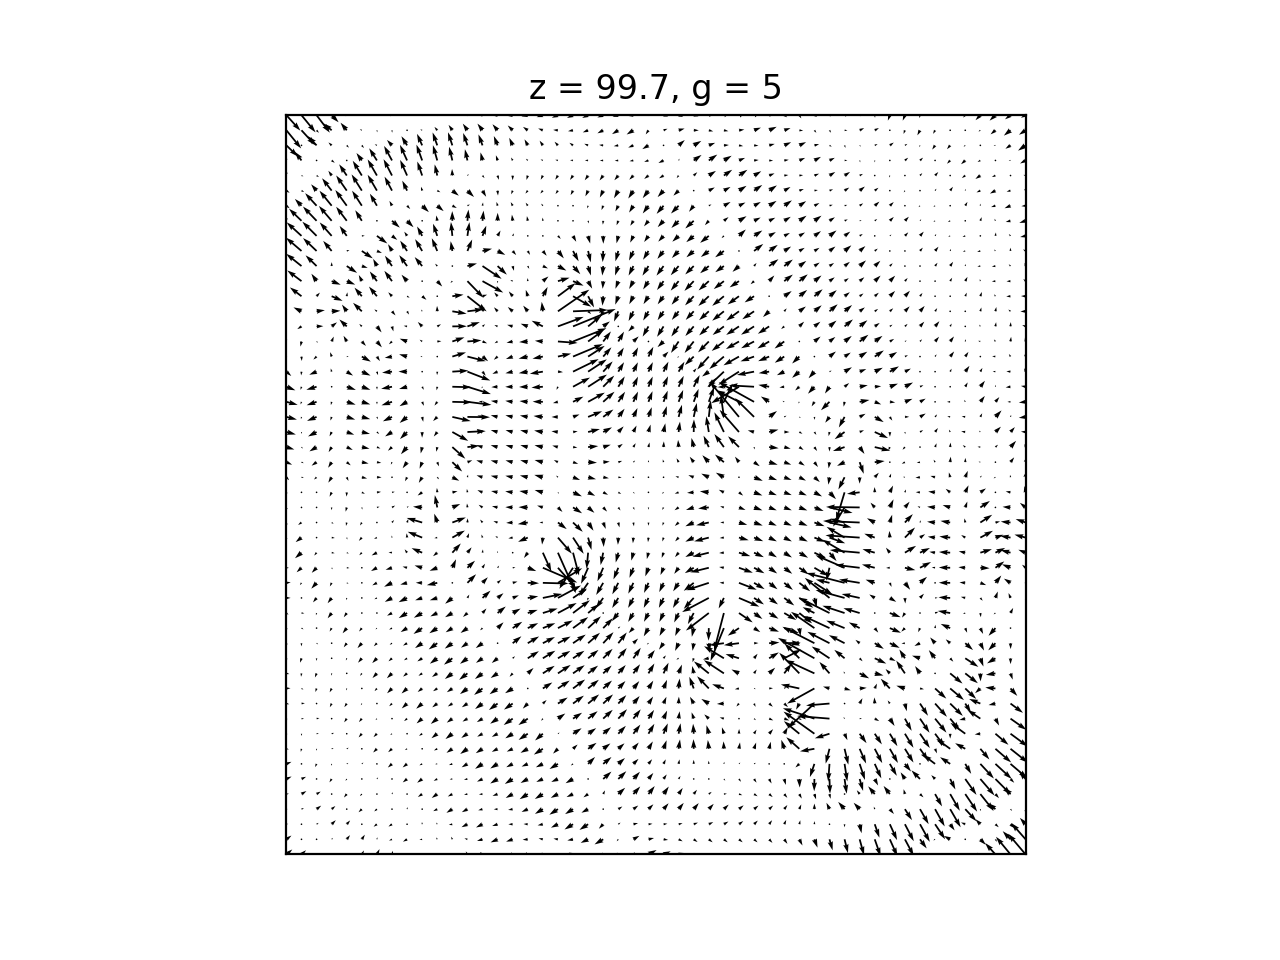
\includegraphics[trim={4cm 0 1cm 0cm},scale=0.5]{vel_99_7_g5.png}
\endminipage\hfill
\minipage{.3\textwidth}
  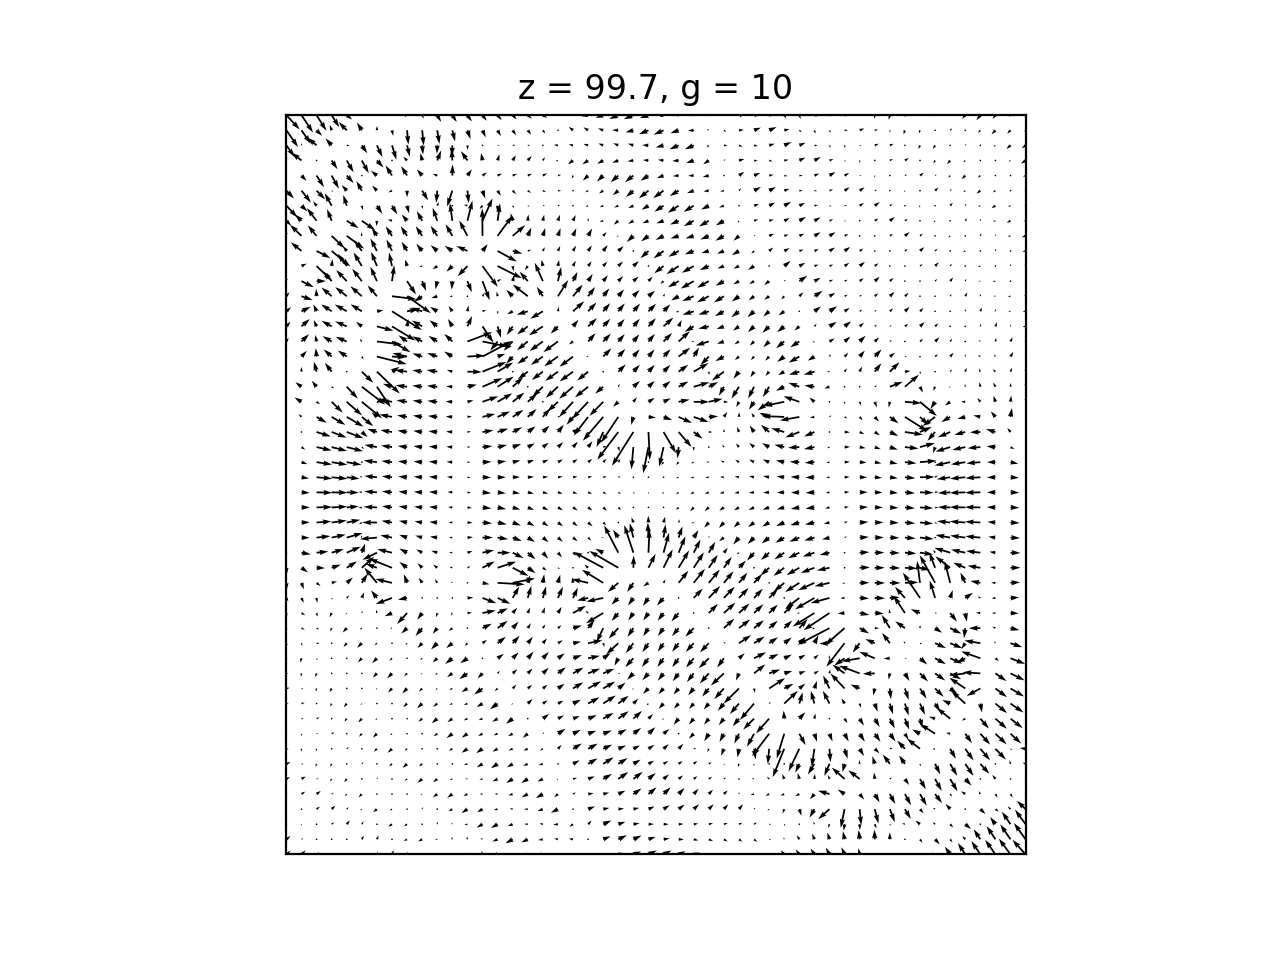
\includegraphics[trim={4cm 0 0cm 0cm},scale=0.5]{vel_99_7_g10.png}
\endminipage\hfill

\minipage{.3\textwidth}
  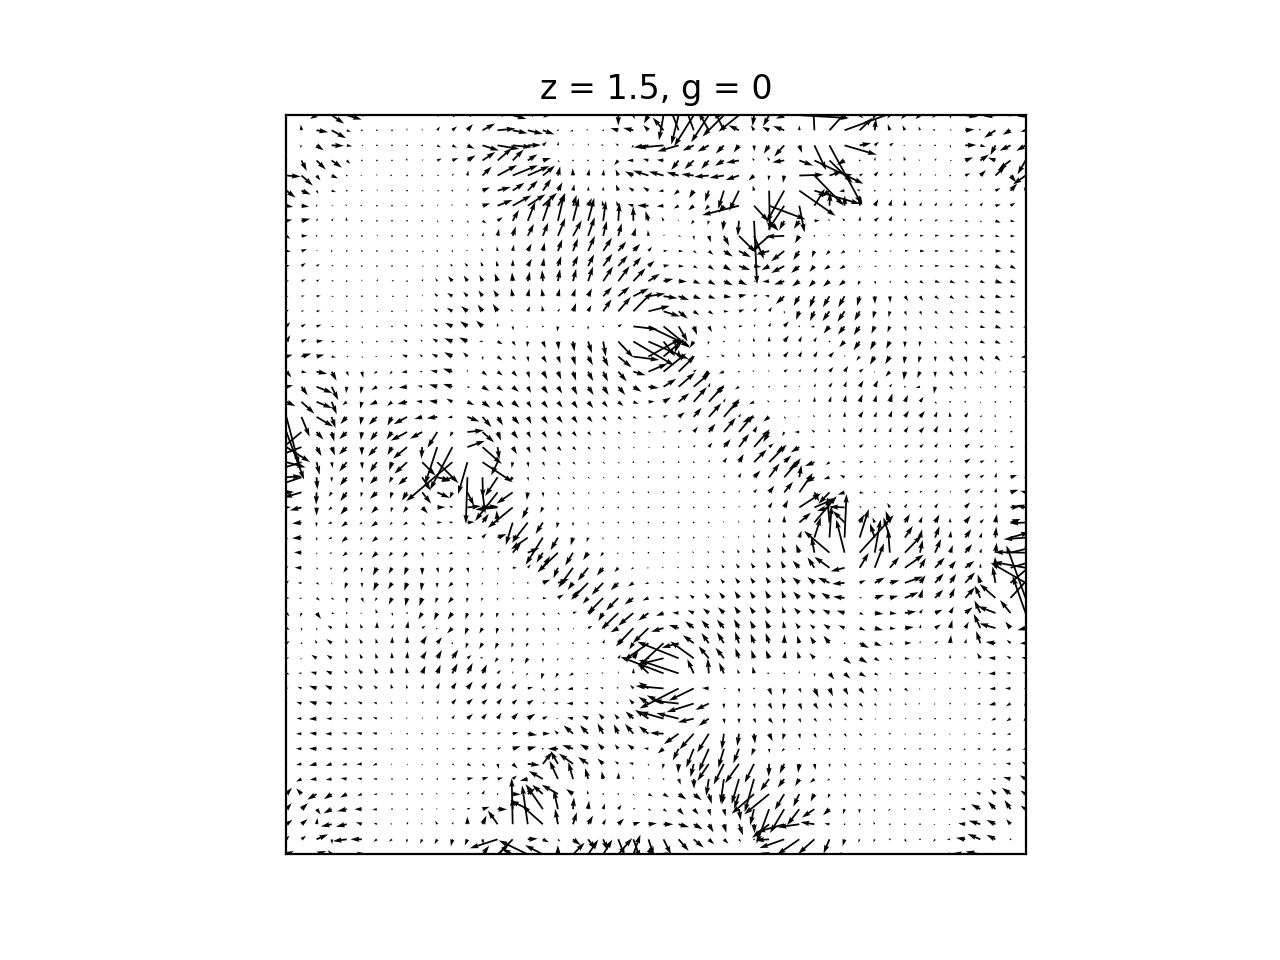
\includegraphics[trim={4cm 0 1cm 0cm},scale=0.5]{vel_1_5_g0.png}
\endminipage\hfill
\minipage{.3\textwidth}
  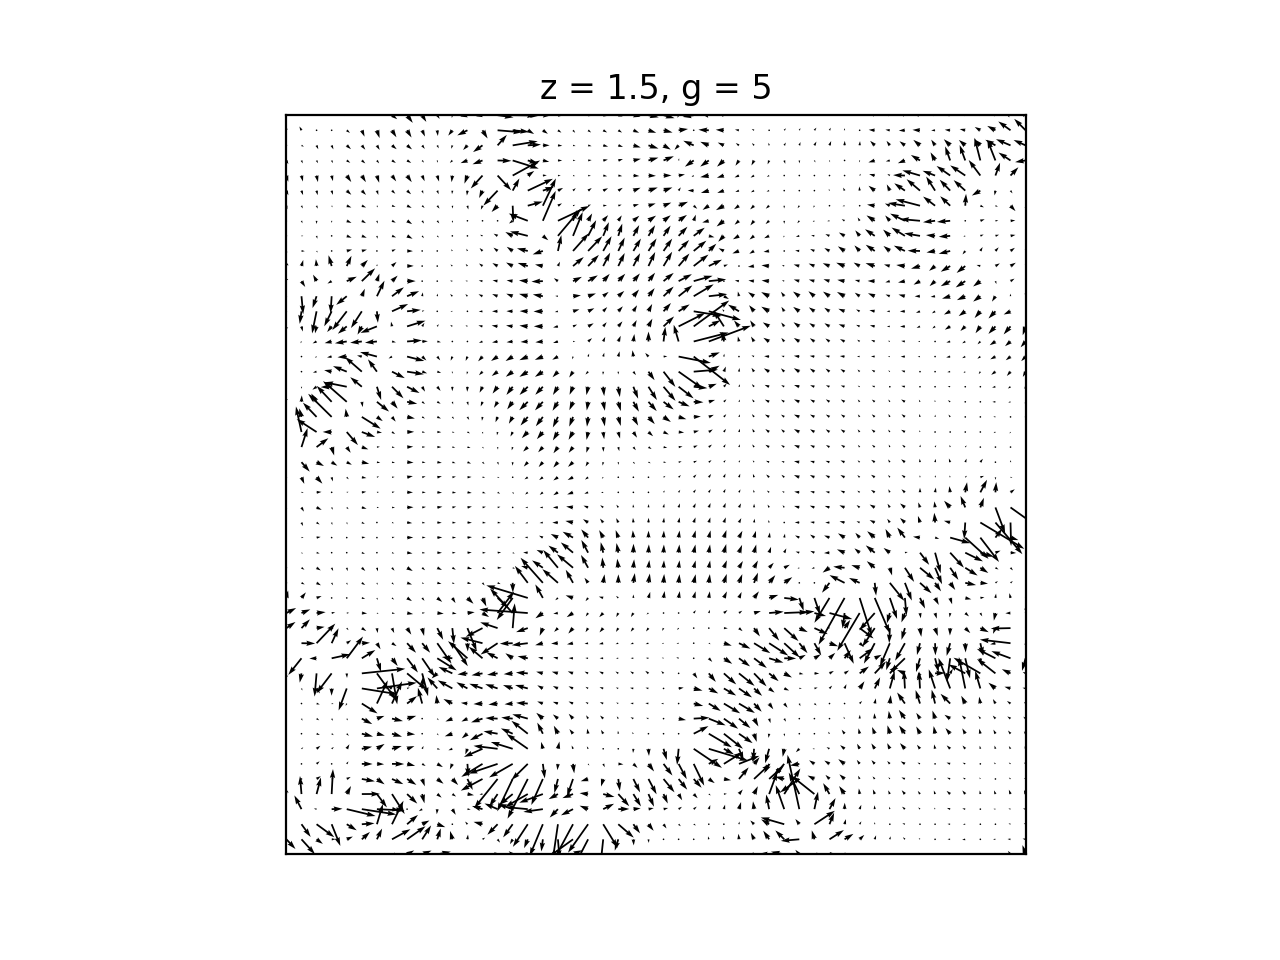
\includegraphics[trim={4cm 0 1cm 0cm},scale=0.5]{vel_1_5_g5.png}
\endminipage\hfill
\minipage{.3\textwidth}
  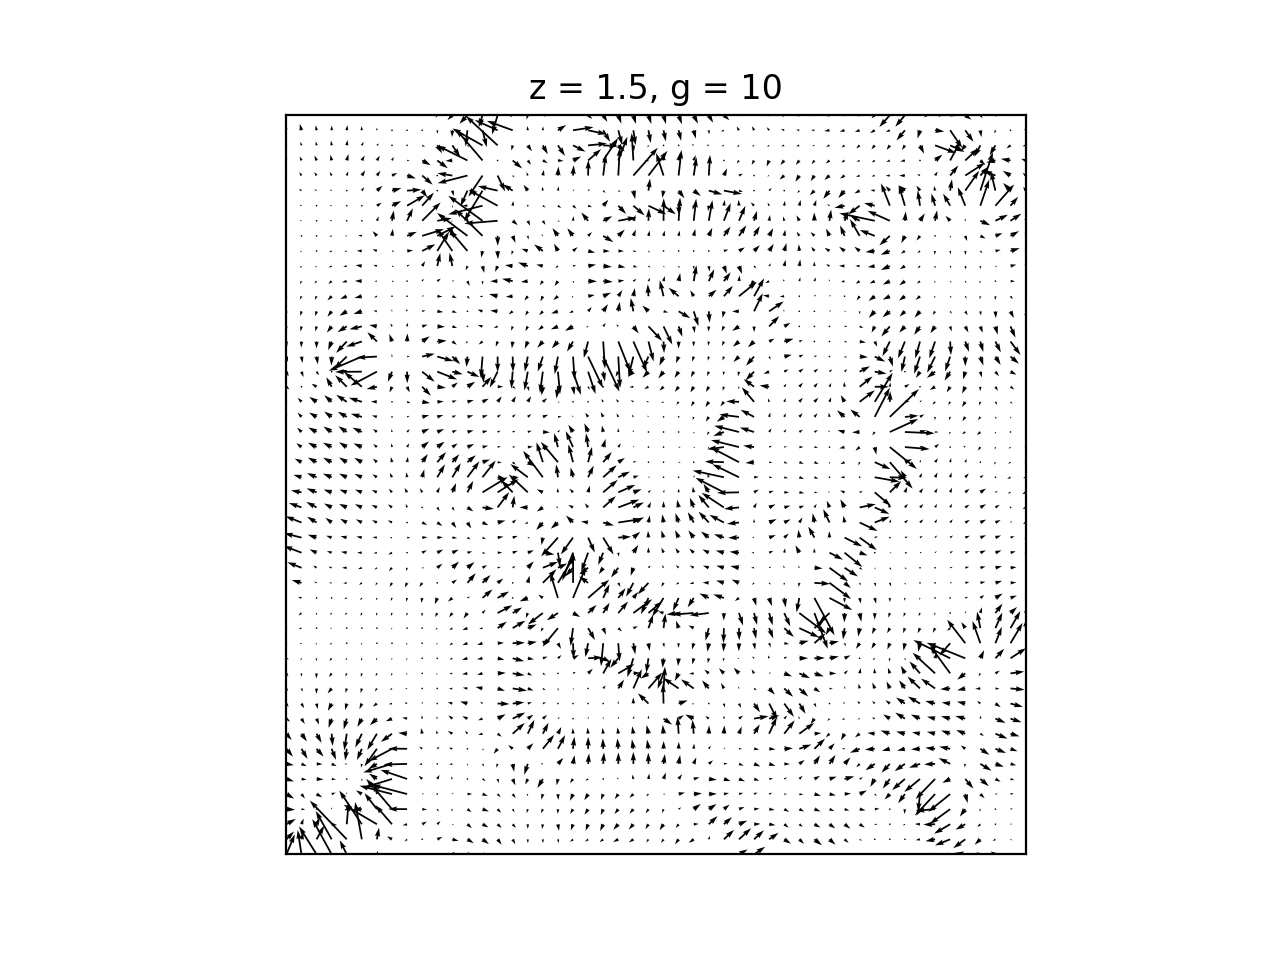
\includegraphics[trim={4cm 0 0cm 0cm},scale=0.5]{vel_1_5_g10.png}
\endminipage\hfill
\caption{Velocity distributions through the centre of the innermost $50^2$ grid points at early ($z = 99.7$, top) and late ($z = 1.5$, bottom) times for increasing $g$.}
\label{fig:vels_initial_final}
\end{figure}

In Figure \ref{fig:vels_initial_final}, we see that at early times in the $g=0$ case, there is a competition between matter infalling under gravitational collapse and outgoing wavefronts due to quantum interference. This initial velocity distribution is clearly distorted due to rotation in the $g=5$ and $g=10$ cases. This in turn results in a proportion of the matter which would otherwise be propagating outward attaining a rotational velocity component, explaining decreased mass loss as $g$ increases. 

At late times, the velocity field in the $g=0$ case is relatively symmetric, and the centre of the grid (surrounding the solitonic core) presents the general features of a Riemann S ellipsoid \cite{Chandrasekhar1965}. As $g$ is increased, the late-time velocity distributions become distorted, indicating complicated dynamics ongoing in the core. This ongoing activity has implications for the core-halo mass relation, particularly in regards to the criteria under which a halo may be considered to be `relaxed'.

We present also a `zoomed-in' version of the late-time velocity fields of Figure \ref{fig:vels_initial_final} in Figure \ref{fig:vels_final_contours}, including a superimposed contour plot of the underlying density distribution. While Figure \ref{fig:profiles_mass_rotation} shows that the spherically-averaged profiles are solitonic, Figure \ref{fig:vels_final_contours} demonstrates anisotropies in the density field, driven by the presence of a non-trivial internal velocity field. Detailed study of the internal velocity fields of halo cores will be undertaken in future work.

\begin{figure}[!htb]
\minipage{.3\textwidth}
  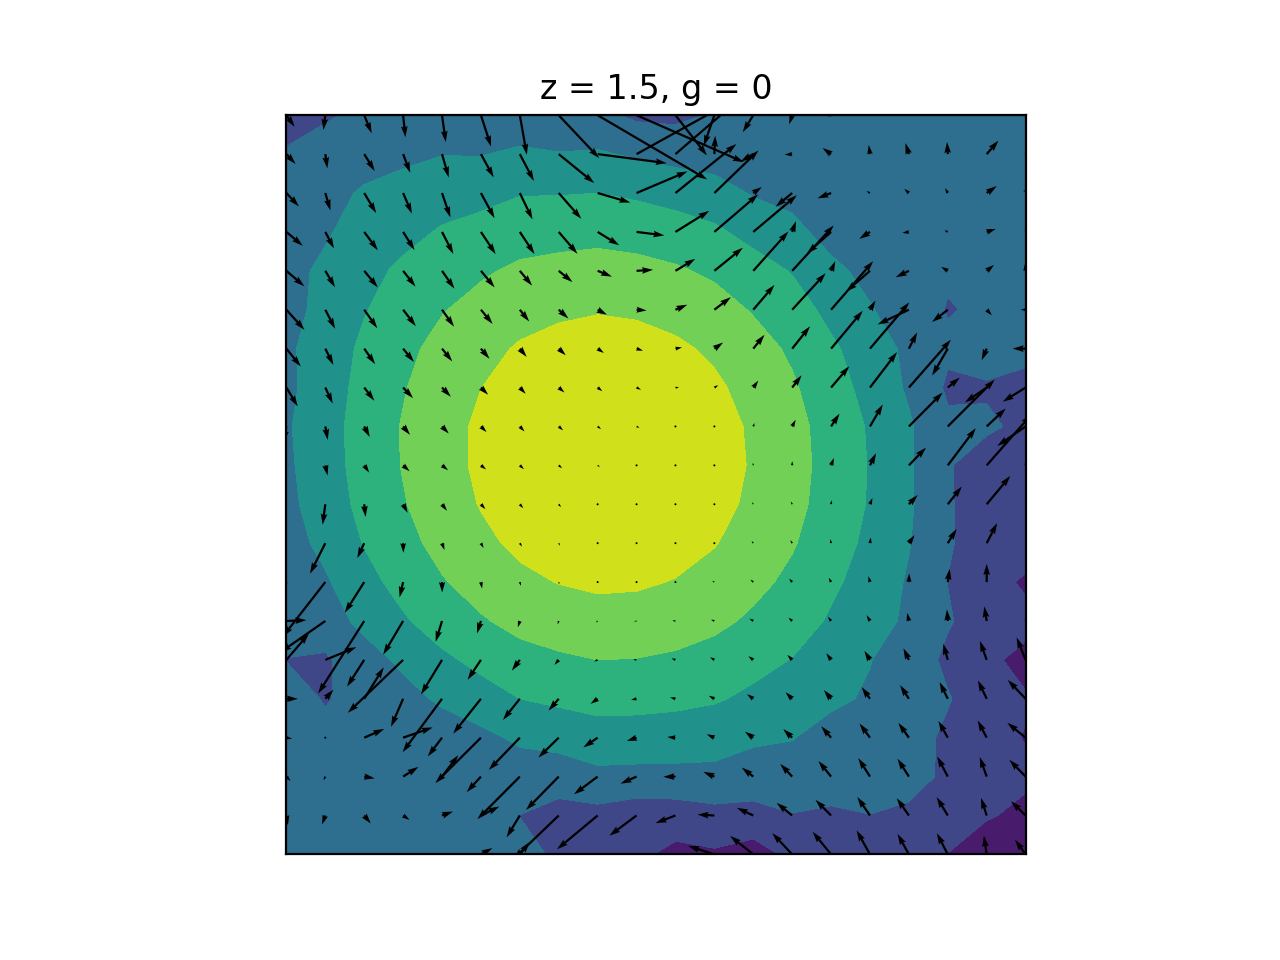
\includegraphics[trim={4cm 0 1cm 0cm},scale=0.5]{small_vel_1_5_g0.png}
\endminipage\hfill
\minipage{.3\textwidth}
  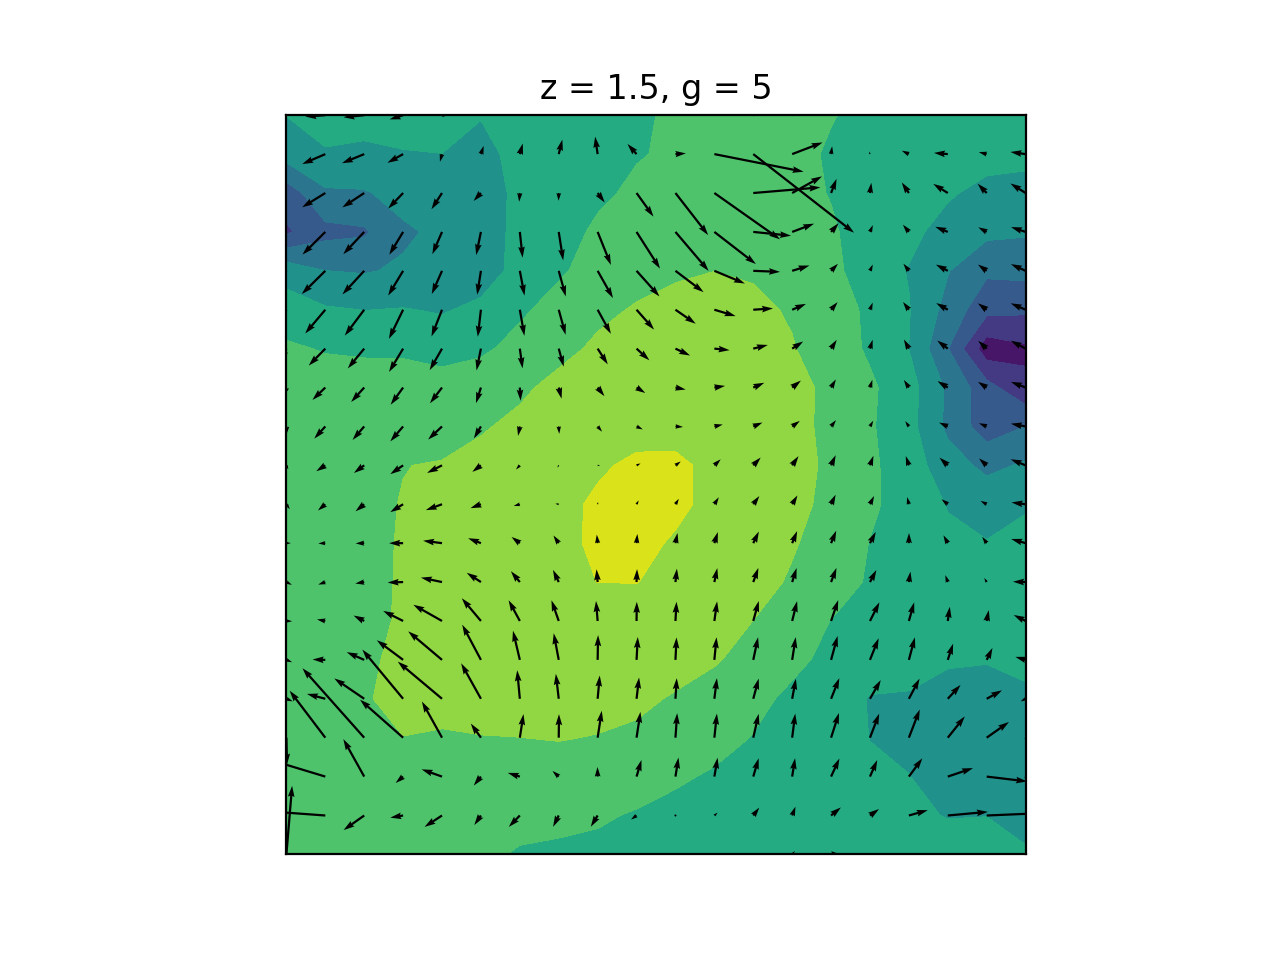
\includegraphics[trim={4cm 0 1cm 0cm},scale=0.5]{small_vel_1_5_g5.png}
\endminipage\hfill
\minipage{.3\textwidth}
  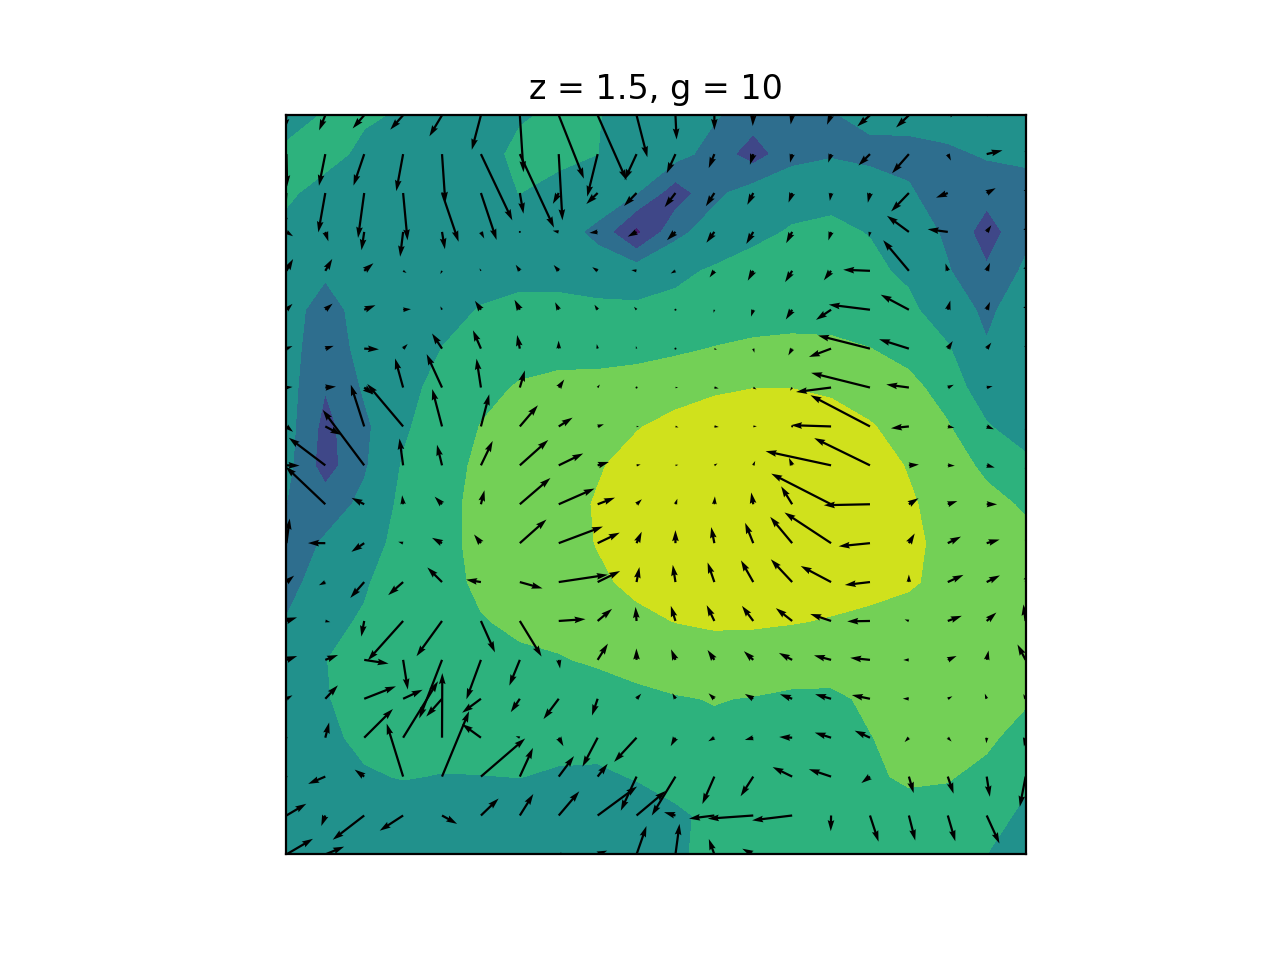
\includegraphics[trim={4cm 0 0cm 0cm},scale=0.5]{small_vel_1_5_g10.png}
\endminipage\hfill

\caption{Velocity distributions through the centre of the innermost $20^2$ grid points at late ($z = 1.5$) time for increasing $g$. Superimposed are density contours.}
\label{fig:vels_final_contours}
\end{figure}





%%%%%%%%%%%%%%%%%%%%%%%%%%%%%%%%%%%%%%%%%%








%%%%%%%%%%%%%%%%%%%%%%%%%%%%%%%%%%%%%%%%%%%%%%%


\section{Conclusions}\label{sec:conclusion}

In this paper we have investigated the collapse of isolated ellipsoidal `top-hat' overdensities in the ULDM model. We find that compared to the Zel'dovich collapse of CDM, collapse of ULDM overdensities is greatly influenced by wave effects and interference processes. We see that the gravitational cooling of relaxing ULDM halos is sensitive not only to ULDM mass, but also to the precise shape of the initial overdensity and the presence of angular momentum. 

We find that variations in the shape and angular momentum of an isolated overdensity can lead to variations in both the rate of mass loss via gravitational cooling, as well as the properties of the final profiles after collapse. In particular, we find evidence for variation around the theoretical prediction for the core-halo mass ratio of ULDM, indicating that the theory may only be valid in the limit of the most symmetric halos with trivial internal velocity distributions. 

We also find that when the initial overdensities are given angular momentum, the final spherically-averaged profiles possess the characteristic core-halo configuration of ULDM, however due to non-trivial variations in the internal velocity field, anisotropies may be present even within the solitonic core which do not show up under spherical averaging. Further investigation of the internal dynamics of ULDM halos will be undertaken in future work using more advanced simulation tools. 

Finally, we also investigated the utility of the traceless tidal tensor as a means by which to characterise the anisotropies in ULDM density distributions arising through wave-like effects on macroscopic scales. We have seen that the probability distributions of the eigenvalues of this tensor exhibit peaks associated with extended filamentary or sheet-like overdensities. The precise position and amplitude of these peaks can be expected to vary with the parameters of the underlying ULDM scalar field, and so we suggest that this could serve as a signature through which to determine the suitability of one model over another. 

Though this work is preliminary in nature, more advanced numerical tools are currently in development which will enable better characterisation of halos and anisotropies within the ULDM model, not just for isolated overdensities, but for large cosmological volumes. The outputs of such detailed simulations can be analysed with the methods employed here in order to obtain a quantitative distinction between different dark matter models. 











\appendix


\section{Code Units}\label{app:units}

The {\sc PyUltraLight} code units are defined by:
\begin{align}
    \CMcal{L}&=\left(\frac{8\pi\hbar^2}{3 m^2H_0^2\Omega_{m_0}}\right)^{\frac{1}{4}}\approx121\left(\frac{10^{-23}\operatorname{eV}}{m}\right)^{\frac{1}{2}}\operatorname{kpc},\label{eq:length}\\
    \CMcal{T}&=\left(\frac{8\pi}{3 H_0^2\Omega_{m_0}}\right)^{\frac{1}{2}}\approx75.5 \operatorname{Gyr},\label{eq:time}\\
    \CMcal{M}&=\frac{1}{G}\left(\frac{8\pi}{3 H_0^2\Omega_{m_0}}\right)^{-\frac{1}{4}}\left(\frac{\hbar}{m}\right)^{\frac{3}{2}}\approx 7\times 10^7\left(\frac{10^{-23}\operatorname{eV}}{m}\right)^{\frac{3}{2}}\operatorname{M}_{\odot}.\label{eq:mass}
\end{align}


\section{Distributions of tidal tensor eigenvalues for density field test cases}\label{app:prob_distro_eg}

To illustrate that overdensities containing extended anisotropic structures correspond to eigenvalue distributions possessing characteristic peaks, we consider two artificial distributions. The first distribution is simply a Gaussian random field, while the second is a 2-dimensional plane wavefront, generated by $\rho(x,y,z)=\sin^2{(x)}$. Figure \ref{fig:gaussian_plane_wave} shows the eigenvalue distributions for the two cases. For the Gaussian random field, in which the statistical fluctuations are isotropic, the eigenvalues themselves are characterised by Gaussian distributions. Meanwhile, the 2-dimensional plane wavefront yields eigenvalue distributions with distinct prominent peaks. The exact position and height of the peaks will of course in general depend on the precise parameters of the waveform.


\begin{figure}[!htb]

\minipage{0.5\textwidth}
  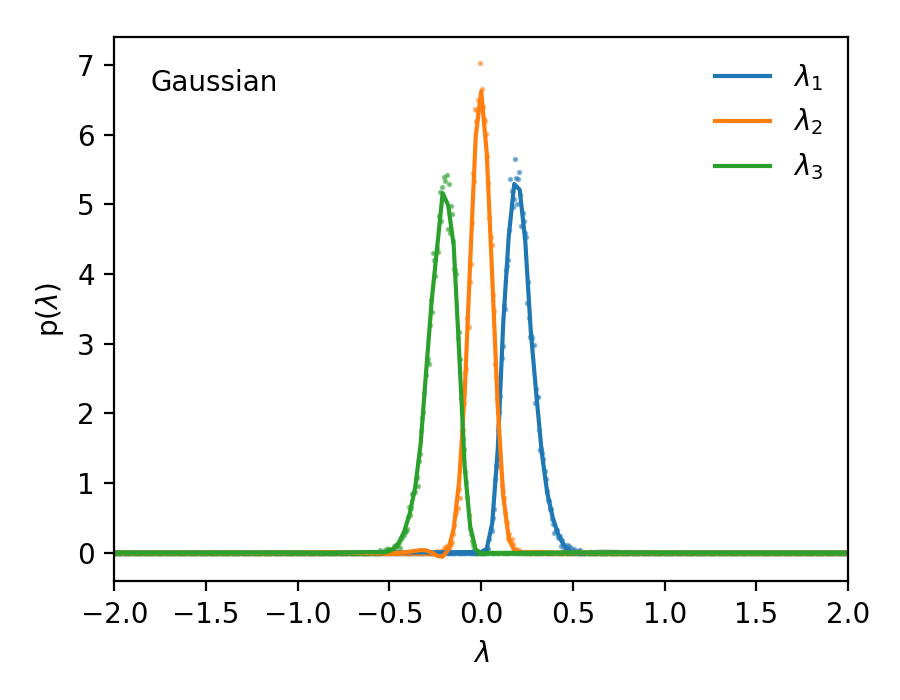
\includegraphics[trim={1cm 0 0 0},scale=0.76]{prob_distro_gaussian.png}
%   \caption{A really Awesome Image}\label{fig:awesome_image2}
\endminipage\hfill
\minipage{0.5\textwidth}%
  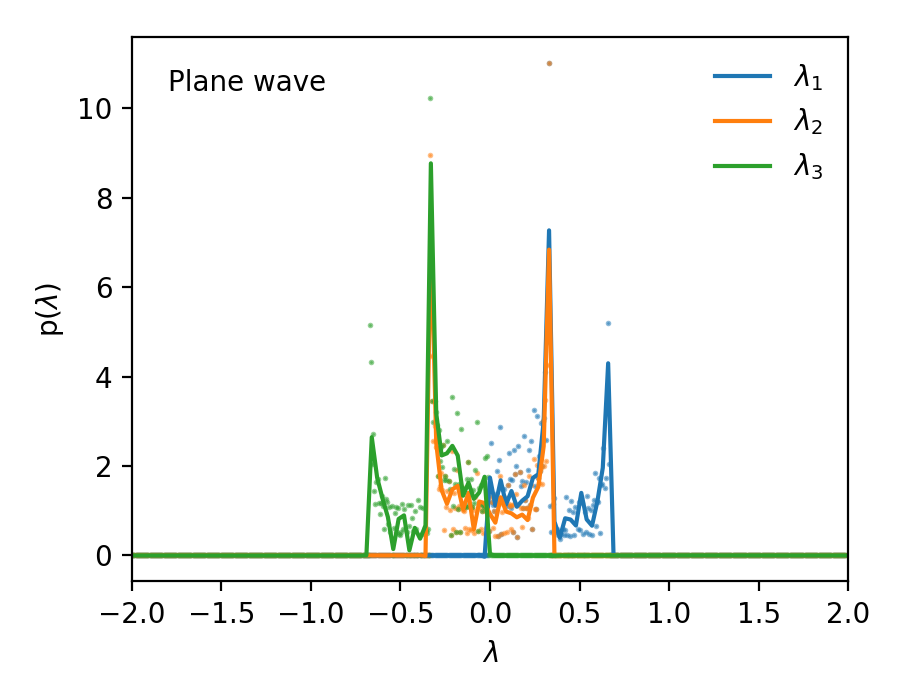
\includegraphics[trim={0cm 0 1cm 0},scale=0.76]{prob_distro_plane_wave.png}

\endminipage
  \caption{Probability distributions of the eigenvalues of the traceless tidal tensor for sample density distributions. Left: Gaussian random field, Right: $\rho(x,y,z) = \sin^2{(x)}$ }\label{fig:gaussian_plane_wave}
\end{figure}







% \acknowledgments

% \paragraph{Note added.} This is also a good position for notes added
% after the paper has been written.





% The bibliography will probably be heavily edited during typesetting.
% We'll parse it and, using the arxiv number or the journal data, will
% query inspire, trying to verify the data (this will probalby spot
% eventual typos) and retrive the document DOI and eventual errata.
% We however suggest to always provide author, title and journal data:
% in short all the informations that clearly identify a document.

\bibliographystyle{JHEP-mod}
\bibliography{refs} 
\end{document}
